% Optional calls for page styles

\documentclass[12pt,letterpaper, openany]{book} %took out one side
%\usepackage[top=2cm, bottom=2cm, lmargin=3.5cm,rmargin=2.5cm,marginparwidth=6cm,marginparsep=2em]{geometry}

%PRINTING FORMAT
\usepackage[top=1.75cm, bottom=1.75cm, lmargin=3.25cm,rmargin=2.25cm,marginparwidth=6cm,marginparsep=2em, twoside]{geometry}

%ONLINE FORMAT
%\usepackage[top=1.75cm, bottom=1.75cm, lmargin=3.25cm,rmargin=2.25cm,marginparwidth=6cm,marginparsep=2em]{geometry}


%\setlength\parindent{0pt} %crush the auto indentation

%Footnote separation
\addtolength{\skip\footins}{1pc}

\reversemarginpar
\usepackage{import}
\usepackage{design}
\usepackage{preamble}

% Watermarking
%\usepackage{draftwatermark}


 
\usepackage{makeidx}
\makeindex


%% Above notes: You can remove twoside and replace with oneside in documentclass to have a better "online pdf" format. twoside is better for printing and binding. You may want to mess with margins to make this better for online viewing.
 
\begin{document}

% WATERMARK
%\SetWatermarkText{Property of Colin Roberts. NOT FOR REDISTRIBUTION.}
%\SetWatermarkColor[gray]{0.75}
%\SetWatermarkFontSize{1cm}
%\SetWatermarkAngle{45}
%\SetWatermarkHorCenter{10cm}
 
\frontmatter
% \noindent\makebox[\textwidth]{\rule{\textwidth}{0.4pt}}

% \huge{Math 255}

% \noindent\makebox[\textwidth]{\rule{\textwidth}{0.4pt}}

\begin{titlepage} % Suppresses headers and footers on the title page

	\centering % Centre everything on the title page
	
	\scshape % Use small caps for all text on the title page
	
	\vspace*{\baselineskip} % White space at the top of the page
	
	%------------------------------------------------
	%	Title
	%------------------------------------------------
	
	\rule{\textwidth}{1.6pt}\vspace*{-\baselineskip}\vspace*{2pt} % Thick horizontal rule
	\rule{\textwidth}{0.4pt} % Thin horizontal rule
	
	\vspace{\baselineskip} % Whitespace above the title
	
	{\LARGE Applied Mathematics for Chemists II} % Title
	
	\vspace{0.3\baselineskip} % Whitespace below the title
	
	\rule{\textwidth}{0.4pt}\vspace*{-\baselineskip}\vspace{3.2pt} % Thin horizontal rule
	\rule{\textwidth}{1.6pt} % Thick horizontal rule
	
	\vspace{2\baselineskip} % Whitespace after the title block
	
	%------------------------------------------------
	%	Subtitle
	%------------------------------------------------
	
	Vector fields, partial differentiation, cylindrical and spherical coordinates, multiple integrals, line integrals, the wave and the Schr\"odinger equations, separation of variables method. Inner Product Spaces. Fourier Series. % Subtitle or further description
	
	\vspace*{3\baselineskip} % Whitespace under the subtitle
	
	%------------------------------------------------
	%	Editor(s)
	%------------------------------------------------
	
	By
	
	\vspace{0.5\baselineskip} % Whitespace before the editors
	
	{\scshape\Large Colin Roberts \\} % Editor list
	
	\vspace{0.5\baselineskip} % Whitespace below the editor list
	
	\textit{Colorado State University} % Editor affiliation
	
	\vfill % Whitespace between editor names and publisher logo
	
	%------------------------------------------------
	%	Publisher
	%------------------------------------------------
	
	%\plogo % Publisher logo
	\begin{figure}[H]
	    \centering
	    
\includegraphics[width=.8\textwidth]{Frontmatter/ram_logo.jpg}
	\end{figure}
	
	\vspace{0.3\baselineskip} % Whitespace under the publisher logo
	
	Created in Spring 2020\\
    Updated in Spring 2021 % Publication year
	
% 	{\large publisher} % Publisher

\end{titlepage}


%No preface for now. Need a new one for 272.
%\section*{Preface}

This text was created to be a companion to the Math 255 - \emph{Calculus for Biological Students II} course at Colorado State University.  The reader is expected to have completed the Math 155 course with a solid grasp of the material in order for one to best absorb new topics in this course.

The aim of this text is to present relevant topics in \emph{multivariate calculus} and \emph{differential equations}.  To begin, one must learn some \emph{linear algebra}. Linear algebra provides a foundation that is required for studying functions of more than one variable.  It is also an extremely beautiful and applicable field of mathematics itself.  Vectors will serve as a generalization of the system of numbers one is already comfortable with.  With vectors, one can study systems that are naturally living in space.  We are already familiar with how functions can be applied to the real numbers, but they can also be applied to vectors living in space.  The simplest types of vector-functions are those that are \emph{linear}.  Given the simplicity, we often wish to understand more complicated functions by investigating their linear approximations.

Calculus studies the rate of change of functions, but it can be rephrased slightly.  Rather, we take the approach that calculus investigates the best linear approximations to functions.  With one variable, a function can be approximated by a tangent line with a slope found by computing the derivative. This is the best linear approximation to a function of one variable.  When functions input and output more than one variable, the derivative is thus a linear function. This slight rewording of the derivative definition allows for the analysis of functions defined in space and time much more naturally.  Of course, we also care about integration. Integration of functions with more than one variable allows for more types of integration.  That is, we can consider integration as a tool to find lengths of curves, areas, volumes, and other physically meaningful quantities.  

Many systems are easier to understand by studying how they change.  For example, if we push an object it accelerates; acceleration is the second derivative of the position function of an object.  In this case, the system is determined by rates of change and so the equation one writes down for this system is a differential equation.  To model systems that change over space and time, one must be able to write down and solve these differential equations.  Physical intuition can help guide one to a solution, but there are more surefire methods.  The main technique proposed is to simplify the problem just enough so that we can solve it more easily but not lose too much information.  Techniques from linear algebra continue to reemerge and allow us to solve a large class of (linear/first order) problems.  Other (nonlinear/higher order) problems can be simplified down to the case we work to solve.  Thus, we create quite a toolbox to investigate differential systems.


 
\clearpage
\thispagestyle{empty}
 
\tableofcontents
 
\mainmatter

\setcounter{part}{4}
\part{Further Topics in Linear Algebra}
\chapter{Hilbert Spaces}
%\section{Introduction}
Recall the importance of the dot product in space.  Given two vectors $\vecu,\vecv \in \R^3$, we defined the dot product by
\[
\vecu \cdot \vecv = u_1v_1 + u_2v_2 + u_3v_3,
\]
and we also referred to this as an inner product.  The dot product allowed us to project a vector onto its components by, for example,
\[
\vecu \cdot \xhat = u_1.  
\]
This was extremely useful for us.  On top of that, the dot product provided us a means of computing the length of a vector by putting
\[
\|\vecu\|=\sqrt{\vecu\cdot\vecu}.
\]
Underlying much of the theory of space was this structure. 

Later, we introduced the Hermitian inner product on complex vectors.  As it turns out, this inner product is strictly more general than the dot product.  If we had two vectors $\veca,\vecb\in \C^n$ (i.e., vectors with $n$ complex number entries) then we defined the inner product by
\[
\langle \veca,\vecb \rangle = \sum_{j=1}^n a_jb_j^*.
\]
Note that if $\veca$ and $\vecb$ only have real entries, then the complex conjugate $b_j^*=b_j$ and we are left with the typical dot product for $\R^n$.  It suffices to say, that we need only care about this Hermitian inner product. In the same vein, we receive all the wonderful benefits of the dot product.  For example, we can project a vector by taking
\[
\xhat_1 = \begin{pmatrix} 1 \\ 0 \\ 0 \\\vdots \\ 0 \end{pmatrix}
\]
and computing
\[
\langle \veca,\vecx_1\rangle = a_1.
\]
Likewise, the length of a complex vector is given by
\[
\|\veca\|=\sqrt{\langle \veca,\veca\rangle}.
\]
Nothing is lost from this more general approach, and this more general approach extends far beyond finite dimensional complex vectors!

\subsection{Infinite Dimensions}

The dimension of a vector is the number of entries needed to fully describe the vector.  From the examples before, we can say that the vectors $\vecu,\vecv\in \R^3$ are 3-dimensional real vectors and the vectors $\veca,\vecb \in \C^n$ are $n$-dimensional complex vectors.  There is no restriction on the size of $n$, and $n$ can in fact be infinite!

This section of the text is primarily concerned with extending our linear algebra techniques to the infinite dimensional case.  Though this may sound ominous, it simply builds upon what we already know.  In essence, we will combine our knowledge of functions, infinite series, integrals, and linear algebra to complete the theory for infinite dimensions.  Put simply, functions will play the role of vectors while series and integrals will play the role of inner products.  This viewpoint places us viewing mathematics from the top, where we can always reduce the general story to something more specific when need be. Ultimately, this allows one to understand one general structure instead of many individual ones.

\section{Function Spaces}

\textcolor{red}{add here}

\section{Inner Products}

Before we define general inner products, let us recall the definition of a vector space.  In the prequel, we had that a vector space $V$ over some field $\field$ (the numbers we choose as entries) is a set containing vectors that satisfy eight different properties.

\begin{exercise}
	Find the definition in the previous text and review it.
\end{exercise}

\begin{df}{Inner Product}{inner_prod_general}
An \boldgreen{inner product} on a vector space $V$ over a field $\field$ is a bilinear (sometimes sesquilinear) function
\[
\innprod{\cdot}{\cdot} \colon V \times V \to \field,
\]
that satisfies
\begin{enumerate}[i.]
	\item (Nondegenerate) For a $\veca\in V$ we have that $\innprod{\veca}{\veca} =0$ if and only if $\veca=\zerovec$;
	\item (Positive definite) For any nonzero $\veca \in V$ we have that $\innprod{\veca}{\veca} > 0$;
	\item (Symmetric) For any $\veca,\vecb\in V$ we have that $\innprod{\veca}{\vecb} = \innprod{\vecb}{\veca}$. If the vector space is complex, then we have conjugate symmetry $\innprod{\veca}{\vecb}=\innprod{\vecb}{\veca}^*$.
\end{enumerate}
What we are denoting is a function $\innprod{\cdot}{\cdot}$ that has two vectors ($V\times V$) as inputs where see $\cdot$ and outputs some number in the designated field $\field$. When we say bilinear, we mean that the function is linear in each input. For example, we have for vectors $\veca,\vecb,\vecc\in V$ and a scalar $\alpha \in \field$ that
\[
\innprod{\alpha\veca + \vecb}{\vecc} = \alpha \innprod{\veca}{\vecc} + \innprod{\vecb}{\vecc},
\]
which shows the linearity in the first input.  The second input is linear as well.

Similarly, if the field $\field=\C$, then the inner product need be sesquilinear in that we instead have the addition of a complex conjugate in the second position. That is, let $\alpha,\beta\in \C$ and we have
\[
\innprod{\alpha\veca + \vecb}{\beta\vecc} = \alpha \beta^*\innprod{\veca}{\vecc} + \beta^*\innprod{\vecb}{\vecc}.
\]
The first position is simply linear.
\end{df}

\begin{exercise}
	Verify that the dot product for $\R^n$ and the Hermitian inner product for $\C^n$ are indeed inner products.
\end{exercise}

Since we have previously covered two different inner products for the finite dimensional vector spaces $\R^n$ and $\C^n$, we can use our intuition from these spaces with their inner product structure to define other important inner products.  We have in fact come across another example while studying the particle in the 1-dimensional box.  Recall that the problem we solved was the equation
\[
-\frac{\hbar^2}{2m} \frac{d^2 \Psi(x)}{dx^2} = E\Psi(x),
\]
on the region $[0,L]$, where $\Psi(x)$ is the wavefunction.  We also imposed the boundary conditions that $\Psi(0)=\Psi(L)=0$ since the particle cannot be found on the boundary of this domain.  

We found that the solutions to this equation were the normalized states 
\[
\psi_n(x) = \sqrt{\frac{2}{L}} \sin\left(\frac{n\pi x}{L}\right),
\]
with corresponding energies $E_n = \frac{n^2h^2}{8mL^2}$. Then, a wavefunction could be written as a linear combination of these states by
\[
\Psi(x) = \sum_{n=1}^\infty a_n \psi_n(x),
\]
where $a_n \in \C$.  In order for the wavefunction $\Psi(x)$ to be normalized, we required that
\[
\sum_{n=1}^\infty \|a_n\|^2=1.
\]
Now, we can consider a set $V$ of all the possible wavefunctions for the above problem as well as the zero function (which is indeed a solution to the problem, but it is not physically meaningful).

\begin{exercise}
	Show that $V$ is a vector space. 
\end{exercise}

We can add an inner product to the vector space $V$ by defining the inner product on two wavefunctions $\Psi$ and $\Phi$ by
\[
\innprod{\Psi}{\Phi} \coloneqq \int_0^L \Psi(x) \Phi^*(x)dx.
\]
To see that this is an inner product, we need to show that the above function is sesquilinear and satisfies the three conditions for an inner product (nondegeneracy, positive definite, and symmetric).  Sesquilinearity follows from the linearity of the integral in that we have
\begin{align*}
	\innprod{\Psi}{\Phi+\alpha \Theta} &= \int_0^L \Psi(x)(\Phi(x)+\alpha \Theta(x))^*dx \\
	&= \int_0^L \Psi(x) \Phi(x)\Phi^*(x)dx+\alpha^* \int_0^L \Psi(x) \Theta^*(x)dx\\
	&= \innprod{\Psi}{\Phi}+\alpha^* \innprod{\Psi}{\Theta}.
\end{align*}
Showing the linearity in the first argument is analogous but there will not be a complex conjugate.  

Next, we can see that the inner product is nondegenerate by noting that if we take the zero function 0, we have
\[
\innprod{0}{0} = \int_0^L 0 dx = 0,
\]
and if we have that
\[
0=\innprod{\Psi}{\Psi}  = \int_0^L \Psi(x)\Psi^*(x)dx = \int_0^L \|\Psi(x)\|^2dx,
\]
it must be that $\|\Psi(x)\|=0$ since this integral cannot be zero otherwise.  Hence, $\Psi(x)$ is the zero function and we have that the inner product is indeed nondegenerate.

By the above work, if $\Psi(x)$ is not the zero function, then $\|\Psi(x)\|^2>0$ and thus we have
\[
\innprod{\Psi}{\Psi}>0.
\]
Hence, the inner product is positive definite.

Lastly, we can see that the inner product is symmetric by taking the Cartesian representation for $\Psi(x)$ by $\Psi(x)=a(x)+ib(x)$ and for $\Phi(x)=c(x)+id(x)$ and noting
\begin{align*}
	\Psi(x)\Phi^*(x) &= (a(x)+ib(x))(c(x)-id(x))\\
		&= (a(x)c(x)+b(x)d(x))+i(b(x)c(x)-a(x)d(x)),
\end{align*}
and
\begin{align*}
	\Phi(x)\Psi^*(x) &= (c(x)+id(x))(a(x)-ib(x))\\
		&= (a(x)c(x)+b(x)d(x))+i(a(x)d(x)-b(x)c(x),
\end{align*}
which means that we have
\[
\innprod{\Psi}{\Phi}=\innprod{\Phi}{\Psi}^*.
\]
Thus we have shown that this is indeed an inner product.

\section{Inner Product Spaces}

Given a vector space $V$ with an inner product, we refer to the vector space as an \boldgreen{inner product space}.  In fact, all the vector spaces we have dealt with are inner product spaces! We tend to prefer working with these spaces as they allow us to nicely compare vectors (like we can with the dot product) and we can also compute lengths and distances.  Needless to say, inner product spaces are immensely important in the physical world.

However, when the vector space is not finite dimensional (such as the space of solutions to the 1-dimensional box with the added zero function), we must be a bit more careful.  Without going into far too much detail, we must add one other attribute to these spaces to make them work as we need.  In this case, we must require that the inner product space is also \boldgreen{complete}.  A space is complete if and only if all Cauchy sequences in the space converge. We call a complete inner product space a \boldgreen{Hilbert space}.

\begin{exercise}
	We defined a Cauchy sequence in the prequel. Find the definition.
\end{exercise}

This extra requirement rules out some oddities and makes the infinite dimensional space much more like the finite dimensional spaces such as $\R^n$ and $\C^n$.  We showed in the prequel that in $\R$ a convergent sequence is also Cauchy. That is, the definitions are analogous. The same happens to be true in $\R^n$ and $\C^n$ (you can picture taking a sequence of vectors instead of a sequence of real numbers).  Thus, in a Hilbert space, Cauchy and convergent are again equal. Let us see why one should believe this.

\begin{ex}{A Cauchy Sequence of Functions}{cauchy_functions}
	Before, we studied power series that define functions.  We would write
	\[
		f(x) = \sum_{n=0}^\infty a_n x^n,
	\]
	where $x$ is in the domain of convergence for the series.  As we worked through what it meant for a series to converge, we found that we could view a series as a sequence of partial sums.  That is, for each value of $x$ we can create a sequence $\{A_n(x)\}_{n=0}^\infty$ by letting
	\[
		A_N(x) = \sum_{n=0}^N a_n x^n.
	\]
	We noted that as we increased $N$, the function $A_N(x)$ became closer and closer to the function $f(x)$.  This was entirely reasonable as if the contrary were true, at some point a large $N$ would provide us a worse approximation to $f(x)$.  

	The completeness assumption for a Hilbert space will give us this ability.  It will allow one to properly approximate quantities such as infinite sums of functions in a way that makes intuitive sense.  
\end{ex}

No more detail is needed on the notion of completeness. We will completely avoid spaces that are not complete as they behave badly.  Take the completeness of any space as given unless it is mentioned otherwise. 

\section{Symmetries}

As previously discussed, symmetry is an important aspect of problem solving that is present in most physical systems.  The prior example is no exception.  We discussed the phase of a complex function and viewed this in an example from quantum mechanics.  There, we found that when a wavefunction is altered by adding a global phase, the probability of making a measurement is not changed.  This is in fact a specific example of something far more general.  But in this case for the particle in the 1-dimensional box, we can see that if alter two wave functions by the same phase and take the inner product
\begin{align*}
\innprod{e^{i\theta} \Psi}{e^{i\theta}\Phi} &= \int_0^L e^{i\theta} \Psi(x) (e^{i\theta}\Phi(x))^*dx \\
	&= \int_0^L e^{i\theta}\Psi(x)e^{-i\theta}\Phi^*(x)dx\\
	&= \int_0^L \Psi(x)\Phi^*(x)dx\\
	&= \innprod{\Psi}{\Phi},
\end{align*}
then the inner product is not changed.  This is an example of a \boldgreen{unitary operator}. A unitary operator preserves the inner product between two vectors. That is, if we have vectors $\Psi$ and $\Phi$ from an Hilbert product space $H$, then $U$ is a unitary operator if $U\colon H \to H$ is onto and
\[
\innprod{U\Psi}{U \Phi} = \innprod{\Psi}{\Phi}.
\]

This is of course not special for just the particle in the 1-dimensional box either. Take the space $\R^2$ with two vectors $\vecu$ and $\vecv$. Then consider a matrix $[A]$ that is in the group $\Orth(2)$ (which means that $[A]$ is a matrix that solely rotates and or reflects vectors).
\begin{exercise}
	Recall the definition of the matrix group $\Orth(2)$.
\end{exercise}
Now, we can actually realize any matrix in $\Orth(2)$ as a reflection matrix, or a product of two reflection matrices. For the sake of example, take a reflection matrix
\[
\REF_\theta = \begin{pmatrix} \cos (2\theta) & \sin(2\theta) \\ \sin(2\theta) & -\cos(2\theta) \end{pmatrix},
\]
which reflects a vector about the line passing through the origin with angle $\theta$ measured from the $x$-axis.  Then letting
\[
\vecu = \begin{pmatrix} u_1 \\ u_2 \end{pmatrix} \qquad \textrm{and} \qquad \vecv = \begin{pmatrix} v_1 \\ v_2 \end{pmatrix},
\]
 we have
\[
\REF_\theta \vecu = \begin{pmatrix} \cos(2\theta)u_1+\sin(2\theta)u_2 \\  \sin(2\theta)u_1-\cos(2\theta)u_2 \end{pmatrix} \qquad \textrm{and} \qquad \REF_\theta \vecv = \begin{pmatrix} \cos(2\theta)v_1+\sin(2\theta)v_2 \\  \sin(2\theta)v_1-\cos(2\theta)v_2 \end{pmatrix}.
\]
\textcolor{red}{Put a picture here}
Then we can compute the inner product of the reflected vectors 
\begin{align*}
\innprod{\REF_\theta \vecu}{\REF_\theta \vecv}&= (\cos(2\theta)u_1+\sin(2\theta)u_2)(\cos(2\theta)v_1+\sin(2\theta)v_2 )\\
&\qquad + (\sin(2\theta)u_1-\cos(2\theta)u_2)(\sin(2\theta)v_1-\cos(2\theta)v_2)\\
&~\vdots\\
&= u_1v_1 + u_2v_2.
\end{align*}
\begin{exercise}
	Show the remaining steps in the above computation.
\end{exercise}
Since this is true for any reflection matrix, it will be true for any product of reflection matrices and hence the group of $\Orth(2)$ matrices are unitary transformations on the inner product space $\R^2$ (where the inner product is the standard dot product).

Every Hilbert space will have a group of unitary symmetries that preserve the inner product. Hence, we tend to have different names for these groups to reflect what the underlying Hilbert product space is. In the particle in a box case, the underlying symmetry is the (slightly inaptly named) unitary group $U(1)$ whereas the case for $\R^2$ it is the orthogonal group $\Orth(2)$.

\section{Bases}

In the case of finite dimensions, we found that we could construct a minimal set of vectors in a space $V$ such that any vector in $V$ can be written as a linear combination of those vectors.  We called such a set a basis.  Take for example, the space $\R^3$, where we had the standard orthonormal basis given by $\xhat$, $\yhat$, and $\zhat$.  We put
\[
\xhat = \begin{pmatrix} 1 \\ 0 \\ 0 \end{pmatrix}, \qquad \yhat = \begin{pmatrix} 0 \\ 1 \\ 0 \end{pmatrix}, \qquad \zhat = \begin{pmatrix} 0 \\ 0 \\ 1 \end{pmatrix},
\]
so that any vector
\[
\vecv = \begin{pmatrix} v_1 \\ v_2 \\ v_3 \end{pmatrix}
\]
could be written as
\[
\vecv = v_1 \xhat + v_2 \yhat + v_3 \zhat.
\]
The latter notation proves to be convenient in the infinite dimensional case.

We have already discovered one way in which we can form a basis for certain infinite dimensional spaces. This came in the form of power series. The major difference is that we have infinite sums to build functions instead of just finite sums to build vectors that live in spaces like $\R^n$ and $\C^n$. 

Let us continue on with the power series example.  For the sake of simplicity, we can consider the space of analytic functions on the region $[0,L]$ (recall that analytic meant the function has a power series).  Then, by definition, every function $f(x)$ in this space can be written as an infinite sum
\[
f(x)=\sum_{n=0}^\infty a_n x^n,
\]
so long as for every $x\in [0,L]$ we have that the above series converges. Thus we have really investigated infinite dimensional spaces and their bases a bit.  In this case, our basis is the set of all powers of $x$. That is to say, we use $\{x^0,x^1,x^2,x^3,\dots\}$ as our basis vectors and the coefficients are the $a_n$.  

In general, the definition of a basis that we have is already correct so long as we understand what it means in general to take a sum. In the previous example with power series, a sum could potentially be infinite.  In some cases (e.g., the Fourier transform) we will see that we may need to take an integral to be our method of summation.  

\subsection{Orthonormal Bases}

Once again, the finite dimensional case led us to discovering the usefulness of an inner product as a method for determining bases that are more useful.  Above, we mentioned the standard orthonormal basis for $\R^3$ which gives us the most natural decomposition of a vector.  Each of the vectors in this basis is of length one and is mutually orthogonal to one another.  Intuitively, this lets you describe a point in space by how much you must walk back or forth, left or right, and up or down to reach your desired location. The orthonormal basis gave us a way to naturally decompose a vector into separate components through the dot product. That is, we could find the $x$, $y$, or $z$-component of a vector and none of these components depend on the others. If you were to take a basis
\[
\vecu = \begin{pmatrix} 1 \\ 1 \\ 0 \end{pmatrix}, \qquad \vecv = \begin{pmatrix} 0 \\ 1 \\ 1 \end{pmatrix}, \qquad \vecw = \begin{pmatrix} 1 \\ 0 \\ 1 \end{pmatrix},
\]
then if you were to break a vector up into these components, you would find that there is some overlap between what each component describes.

\begin{exercise}
	Show the vectors $\vecu$, $\vecv$, and $\vecw$ above form a basis.  Then, to see that there is some overlap, you can find the components of a vector (of your choice) in the directions $\uhat$, $\vhat$, and $\what$. \emph{Hint: to see the overlap, determine the length of the vector you chose, and compare it to the length computed from components un the $\uhat$,$\vhat$, and $\what$.}
\end{exercise}

When a basis is not orthogonal, then to find independent components of a vector, you must somehow subtract off the overlap. This process is a bit tedious, so instead of giving an example, we can just assert the fact that orthogonal bases are indeed helpful. 

\begin{remark}
	Orthogonal bases in finite dimensions also appear when we find eigenvalues and eigenvectors for Hermitian matrices. Specifically, the set of eigenvectors corresponding to different eigenvalues for a Hermitian matrix are always orthogonal!
\end{remark}

One may wish that the Hilbert spaces would have some sense of a natural decomposition into different orthogonal components.  It turns out that in the realm of spaces we care about we can do this, and that some Hilbert spaces have particularly nice bases to work with. In the prequel, we studied series solutions to differential equations as a means of solving a large class of equations. During that time, we solved Legendre's equation and found the solutions were particularly nice.

Recall the equation we wished to solve was
\[
(1-x^2)f''(x)-2xf'(x)+m(m+1)f(x)=0
\]
with our domain $\Omega=[-1,1]$ and $m$ a non-negative integer ($m=0,1,2,\dots$). Ignoring the details, we found that there were solutions for each $m$ (which in some sense are like the eigenvalues for the 1-dimensional box).  The normalized solutions were known as the Legendre polynomials and the first few were
\begin{align*}
	f_0(x)&=\sqrt{\frac{1}{2}} & f_1(x)&=\sqrt{\frac{3}{2}} x\\
	f_2(x)&= \sqrt{\frac{5}{8}} (1-3x^2) & f_3(x)&=\sqrt{\frac{63}{8}}\left(x-\frac{5x^3}{3}\right).
\end{align*}
One may be wondering what we mean by normalized here. The solutions to the Legendre equation live in a Hilbert space whose inner product is given by
\[
\innprod{\Psi}{\Phi} = \int_{-1}^1 \Psi(x)\Phi(x)dx,
\]
in which these functions are normalized. That is, we have  
\[
\|f_i\|= \sqrt{\innprod{f_i}{f_i}} = 1,
\]
for every $i$. Note we do not need a complex conjugate in this inner product since these functions are all real valued. Moreover, it turns out that this set of polynomials is orthonormal since we also have
\[
\innprod{f_i}{f_j} = 0
\]
if $i\neq j$. Finally, the Legendre polynomials form a basis for the solution to the Legendre equation.  Specifically, we can write any other solution as a series of Legendre polynomials by
\[
f(x)= \sum_{n=1}^\infty a_n f_n(x),
\]
so long as the series converges for all values of $x$ in the domain $\Omega$.  

In the realm of quantum mechanics, the orthonormal basis of eigenfunctions are extremely important. Previously, we even donated these functions with the term \boldgreen{states}.  Though we never defined this term in the prequel, we now have a rough working definition.  When observing a quantum system, it is only possible to observe a particle in an eigenstate of the operator that is mathematical representation for the observation you are wishing to make.  We will define operators, eigenfunctions, and observables later.

\subsection{Expansion and Projection}



\chapter{Linear Operators}
%fourier transforms?
spectral theory with fourier and with 1st and second order derivatives and matices. different domains for different spectra, schrodinger equation with quadratic potential QHO.  Start with complex functions since they introduce multivariate functions and inner products nicely. Can talk about U(1)?

\part{Multivariate Calculus}
\chapter{Functions}
   
        \section{Overview of multivariate functions}
        Now that we have covered enough of the complex numbers, we will move back into the vector space $\R^n$ and analyze the types of functions we can have with this space.  Specifically, we will concentrate on $\R^3$ (or $\R^2$) and functions of the form:
        \begin{align}
            &\gamma\colon \R \to \R^3\\
            &f\colon \R^3 \to \R\\
            &\mathbf{v}\colon \R^3 \to \R^3.
        \end{align}
        Abstractly, I could call each one of these functions a \emph{field} (in the physics sense).  However, I'll refrain from this (and let the mathematicians breathe a sigh of relief).
        
%        
%        \begin{enumerate}[(1)]
%        \item Functions of the form
%        \[
%        \gamma \colon \R\to \R^3
%        \]
%        are \textbf{curves}.  Often times, we will have 
%        \[
%        \gamma \colon [a,b]\to \R^3
%        \]
%        when we want curves with specific endpoints. We will concentrate first on curves, so I'll save the extra detail for a bit later.
%        
%        \item Functions of the form
%        \[
%        f\colon \R^3 \to \R
%        \]
%        are \textbf{scalar fields} or \textbf{scalar functions}.   These functions are useful in describing quantities like temperature in space.  At each point in space $\R^3$, we can assign a single number $\R$ that tells us this temperature.  One may ask how this function changes from point to point.  Asking this question sends you immediately to investigating the \emph{gradient}.  It turns out, using our temperature example, that we can understand heat flow by understanding temperature gradients.
%        
%        \item Functions of the form
%        \[
%        \mathbf{v}\colon \R^3 \to \R^3
%        \]
%        are called \textbf{vector fields}.  Roughly speaking, at each point in space $\R^3$, we can place a vector that is also in $\R^3$.  These fields are very important in describing systems that have flow.  For example, fluid flow or electromagnetism are vector field theories.  What will it mean to find the change in a vector field?  This will lead us to the notion of the \emph{total derivative}.  This concept is a bit abstract at first but will really tell us the proper notion of the derivative.
%        \end{enumerate}
%        
%        \section{Curves in space}
%        
%        We will begin these multivariate functions by considering functions that are not multivariate!  Why? Because curves are very much useful tools and this will help us visualize results for the other types of functions.
%        
%        Let us consider a curve
%        \[
%        \gamma \colon \R \to \R^3.
%        \]
%        We will specify a specific curve by supplying three functions $f_1(t)$, $f_2(t)$, and $f_3(t)$. Specifically, each of these functions $f_i$ is a function $f_i\colon \R \to \R$. Then, we can say that
%        \[
%        \gamma(t)=(f_1(t),f_2(t),f_3(t))=\begin{bmatrix} f_1(t)\\ f_2(t)\\ f_3(t)\end{bmatrix}.
%        \]
%        \emph{Note, I will likely use these above notations for vectors interchangeably.} 
%        
%        Each $f_i(t)$ (for the values $i=1,2,3$) is called a \textbf{coordinate function}.  Intuitively, the coordinate function tells us where the curve is at a time $t$. That is
%        \begin{align*}
%            &f_1(t) \quad \textrm{the $x$-position of $\gamma$ at time $t$,}\\
%            &f_2(t) \quad \textrm{the $y$-position of $\gamma$ at time $t$,}\\
%            &f_3(t) \quad \textrm{the $z$-position of $\gamma$ at time $t$.}
%        \end{align*}
%        The nice thing about these coordinate functions is we entirely know how to deal with their calculus since each is a function $f_i\colon \R \to \R$.
%        
%        Now, we can find the \textbf{tangent vector} or \textbf{velocity vector} to the curve $\gamma$ at a time $t$.  We covered this in the complex case, and the idea here is arguably more straightforward. 
%        
%        Imagine that $\gamma(t)$ is the position of a small particle at the time $t$.  Then the velocity is the time rate of change of this position.  Specifically, we see how each of the coordinate functions changes, and this will tell us how the position changes! So, we have the following.
%        
%        \begin{df}{Tangent Vector to a Curve}{tang_to_curve}
%        Given a curve $\gamma$, the \textbf{tangent vector to $\gamma$ at the time $t$} is
%        \[
%        \gamma'(t)=\lim_{\delta \to 0} \frac{\gamma(t+\delta)-\gamma(t)}{\delta}.
%        \]
%        It turns out that we find $\gamma'$ is
%        \[
%        \gamma'(t)=(f_1'(t),f_2'(t),f_3'(t))=\begin{bmatrix} f_1'(t)\\ f_2'(t)\\ f_3'(t)\end{bmatrix}.
%        \]
%        \end{df}
%        
%        \begin{ex}{Graph of a Quadratic Function}{graph_quad}
%        Consider the curve $\gamma\colon \R \to \R^2$ given by
%        \[
%        \gamma(t)=(t,t^2).
%        \]
%        This curve looks exactly like the graph of the function $f(x)=x^2$ that we have drawn many times before. 
%        \begin{figure}[H]
%            \centering
%            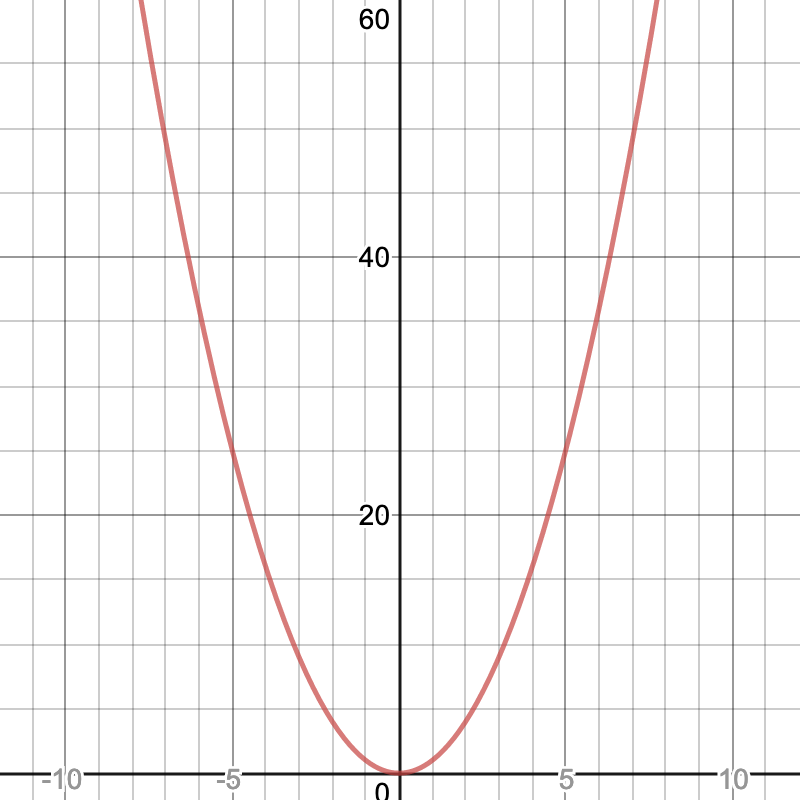
\includegraphics[width=.4\textwidth]{Figures/quadratic_curve.png}
%        \end{figure}
%        
%        What is the tangent vector at time $t$? We have
%        \[
%        \gamma'(t)=(1,2t).
%        \]
%        If we take this $y$-value over the $x$-value we arrive at the same conclusion for the derivative to $f(x)=x^2$ (i.e., $f'(x)=2x$).
%        \end{ex}
%        
%        \begin{ex}{Circle Curve}{circ_curve}
%        Consider the curve $\gamma \colon [0,1] \to \R^2$ given by
%        \[
%        \gamma(t)=(\cos (2\pi t),\sin (2\pi t)).
%        \]
%        This curve is a circle of radius $1$ centered at $(0,0)$.  We can find the tangent vector at a time $t$ by
%        \[
%        \gamma'(t)=(-2\pi \sin(2\pi t), 2\pi \cos(2\pi t)).
%        \]
%        See the following graphs
%        
%    \begin{figure}[H]
%    \centering
%    \begin{subfigure}[h]{0.45\textwidth}
%        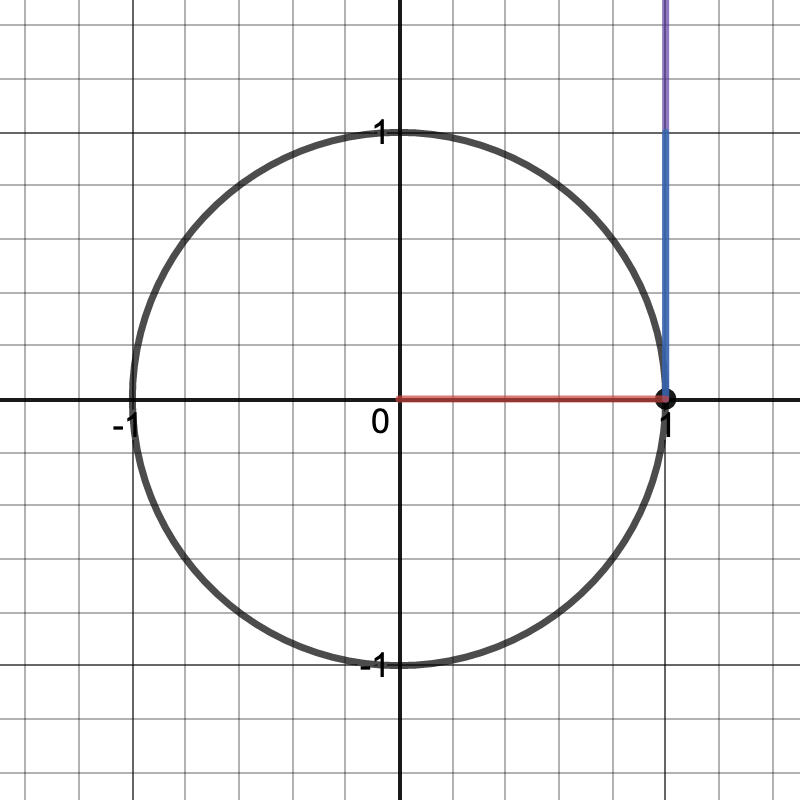
\includegraphics[width=\textwidth]{Figures/circ_tang_1.png}
%        \caption{Tangent vector at $t=0$.}
%    \end{subfigure}
%    ~ 
%    \begin{subfigure}[h]{0.45\textwidth}
%        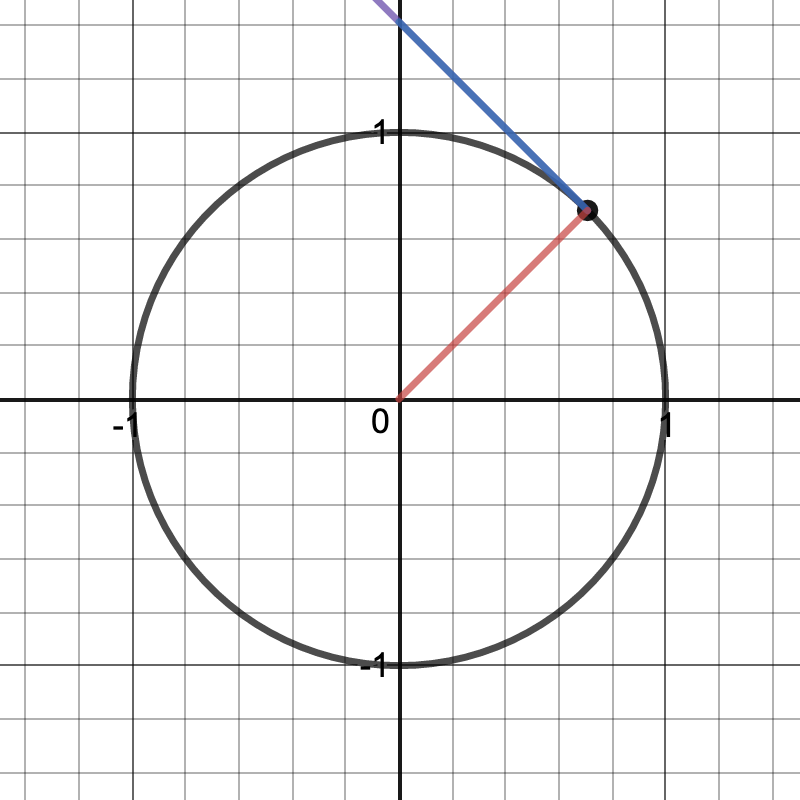
\includegraphics[width=\textwidth]{Figures/circ_tang_2.png}
%        \caption{Tangent vector at $t=\frac{1}{8}$.}
%    \end{subfigure}
%    
%    \begin{subfigure}[h]{0.45\textwidth}
%        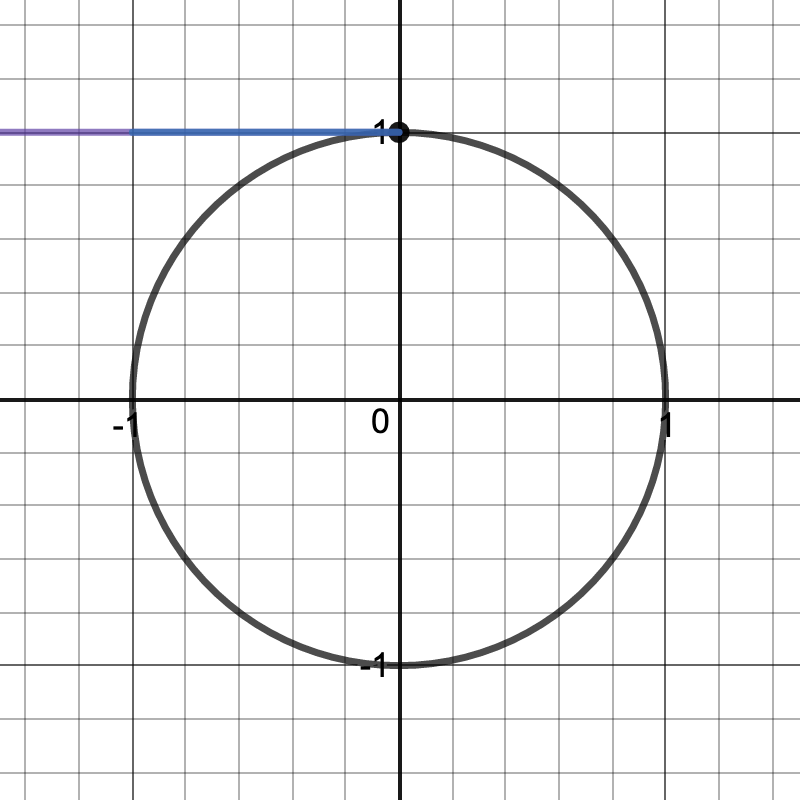
\includegraphics[width=\textwidth]{Figures/circ_tang_3.png}
%        \caption{Tangent vector at $t=\frac{1}{4}$.}
%    \end{subfigure}
%    ~
%    \begin{subfigure}[h]{0.45\textwidth}
%        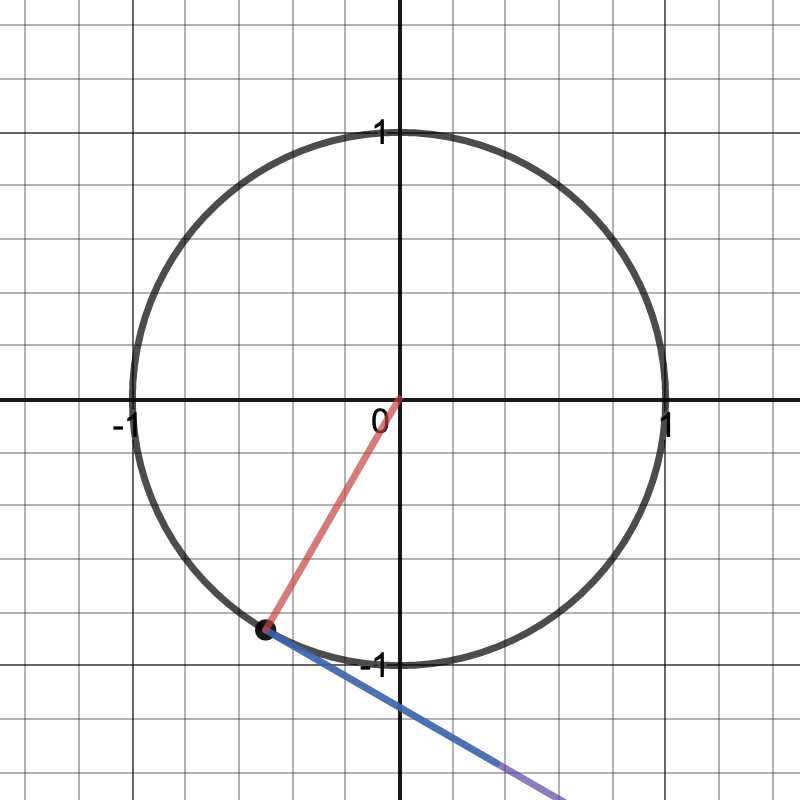
\includegraphics[width=\textwidth]{Figures/circ_tang_4.png}
%        \caption{Tangent vector at $t=\frac{2}{3}$.}
%    \end{subfigure}
%        \end{figure}
%        
%        We can also compute the \textbf{normal vector} or \textbf{acceleration vector} to a curve by taking another derivative.  We write
%        \[
%        \gamma''(t)=(-4\pi^2 \cos(2\pi t),-4\pi^2 \sin(2\pi t)).
%        \]
%        \end{ex}
%        
%        \subsubsection{Line integrals}
%        
%        In reality, we like to add up function values along curves.  We have already done this before in the complex case with contours.  You also did this in a calculus I course via the Riemann integral.  We will get to this, but we need to know the correct functions to add up along a curve first. These will be the vector and scalar fields fields.
%        
%        
%        
%        \section{Scalar fields}
%        The next major class of functions we will consider are the scalar fields.  That is, functions that take the form
%        \[
%        f\colon \R^3 \to \R.
%        \]
%        Often, it will be helpful to visualize functions by considering instead
%        \[
%        f\colon \R^2 \to \R
%        \]
%        and looking at the \emph{graph} of $f$.  
%        
%        \begin{ex}{Graph of a function}{graph_of_func}
%        Whenever we talk of a function of the form
%        \[
%        f\colon \R \to \R
%        \]
%        we inherently tend to draw the graph of the function $f$.  By graph, I mean that given $f$, we usually just draw $(x,f(x))$ in the plane.
%        
%        Take for example, $f\colon \R \to \R$ given by $f(x)=x^2$.  We usually draw the plane $\R^2$ and graph the curve $(x,f(x))$ which looks like
%        \begin{figure}[H]
%            \centering
%            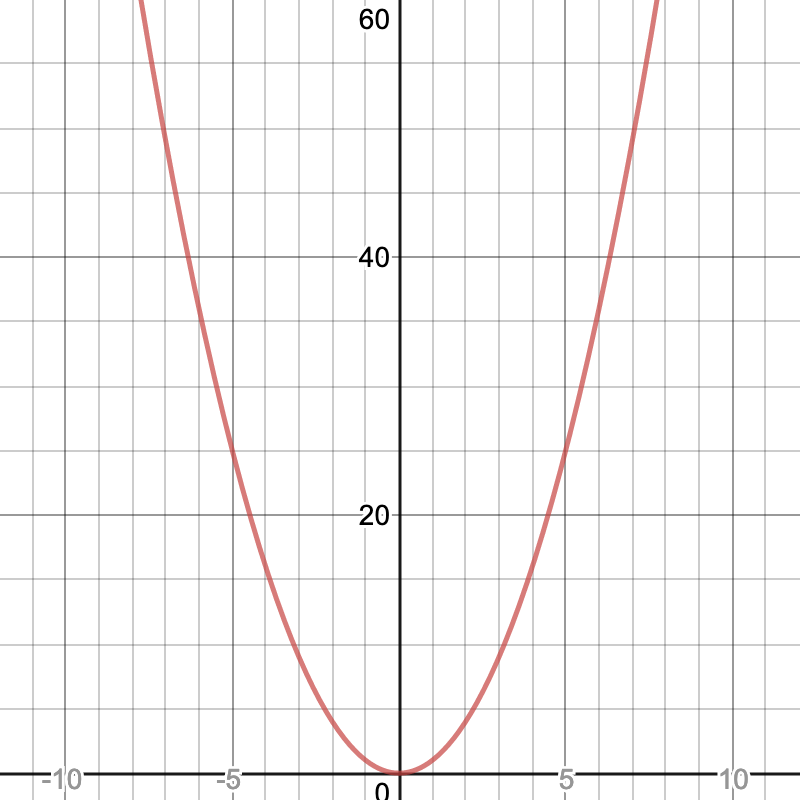
\includegraphics[width=.5\textwidth]{Figures/quadratic_curve.png}           
%        \end{figure}
%        All of this is to say that graphs of these types of functions are special kinds of curves.  In other words, they are curves that pass the vertical line test.
%        \end{ex}
%        
%        \begin{ex}{The Paraboloid}{paraboloid}
%        Let $f\colon \R^2 \to \R$ be given by
%        \[
%        f(x,y)=x^2+y^2.
%        \]
%        We can plot the graph of the function by plotting $(x,y, f(x,y))$ in $\R^3$.  This will look like:
%        \begin{figure}[H]
%            \centering
%            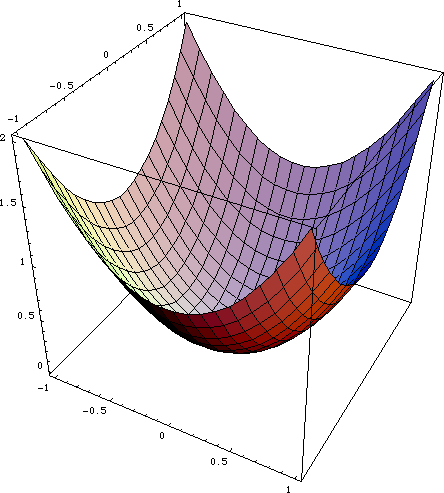
\includegraphics[width=.4\textwidth]{Figures/paraboloid.png}
%        \end{figure}
%        Then we can analyze this function in a few nice ways.  
%        
%        If we fix a value for $x$ or $y$, then we will be able to look at $f$ as a function of just a single variable.  
%        \begin{itemize}
%        \item So we can, for example, fix $y=0$ and then we have
%        \[
%        f(x,0)=x^2.
%        \]
%        So along the $y=0$ line, the function is just the parabola we are used to! 
%        
%        \item Similarly, we can force $x=0$ and arrive at
%        \[
%        f(0,y)=y^2
%        \]
%        is also a parabola.  
%        
%        \item But we are not limited to these choices.  We could have chosen $y=5$ and we would have
%        \[
%        f(x,5)=x^2+25
%        \]
%        which is a parabola shifted upwards by 25 units.
%        
%        \item  Again, we could also choose yet another ``slice" of this function and let $x=y$ which would give us
%        \[
%        f(x,x)=x^2+x^2=2x^2.
%        \]
%        So, along the $x=y$ line, the parabola is scaled by 2.
%        
%        \item One other method of analyzing this function would be to find what the \textbf{level curves} of this function are.  What are the points $(x,y)$ that satisfy $f(x,y)=c$?  We call these level curves much in the way that a topographical map plots curves along the areas with equal height.  For this example, consider the set of points $(x,y)$ so that $f(x,y)=1.$ This means
%        \[
%        f(x,y)=1=x^2+y^2.
%        \]
%        Since we have
%        \[
%        x^2+y^2=1
%        \]
%        that means each level curve is a circle!
%        \item Here is a ``topographical map" for this function (i.e., a plot of the level curves for this paraboloid.)
%        \begin{figure}[H]
%            \centering
%            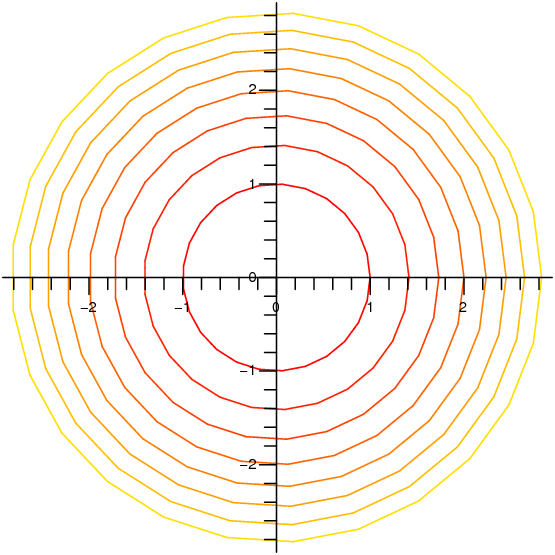
\includegraphics[width=.4\textwidth]{Figures/parabolic_level_curves.png}
%        \end{figure}
%        Here, each circle represents $f(x,y)=c$ for different values of $c$.  This really \emph{is} a topographical map!
%        \end{itemize}
%        \end{ex}
%        
%        \begin{exercise}[Plane]
%        Repeat this analysis for yourself for the following function:
%        \[
%        f(x,y)=x+y.
%        \]
%        \end{exercise}
%        
%        \section{Level surfaces}
%        In the planar case, we would often have to specify a set of points like
%        \[
%        x^2+y^2=1
%        \]
%        which is the circle.  
%        
%        In higher dimensions, we can do the same in order to visualize functions of the form $f\colon \R^3\to \R$ written as $f(x,y,z)$.  If we pick some constant $c$ and write
%        \[
%        f(x,y,z)=c
%        \]
%        then we will get the \textbf{level surfaces} for the function $f(x,y,z)$.  Visualizing functions of three variables (or more) $f(x,y,z)$ requires us to visualize in four or more dimensions. So we often reduce the problem to visualizing level surfaces.
%        
%        \begin{ex}{A Sphere as a Level Surface}{sphere_lev_surf}
%        We can consider the following function
%        \[
%        f(x,y,z)=x^2+y^2+z^2.
%        \]
%        If we take the one level set, that is the points $(x,y,z)$ that satisfy
%        \[
%        x^2+y^2+z^2=1
%        \]
%        then we get the \emph{2-sphere}.  These are the set of points that are all a distance one from the origin.  Here is a picture:
%        \begin{figure}[H]
%            \centering
%            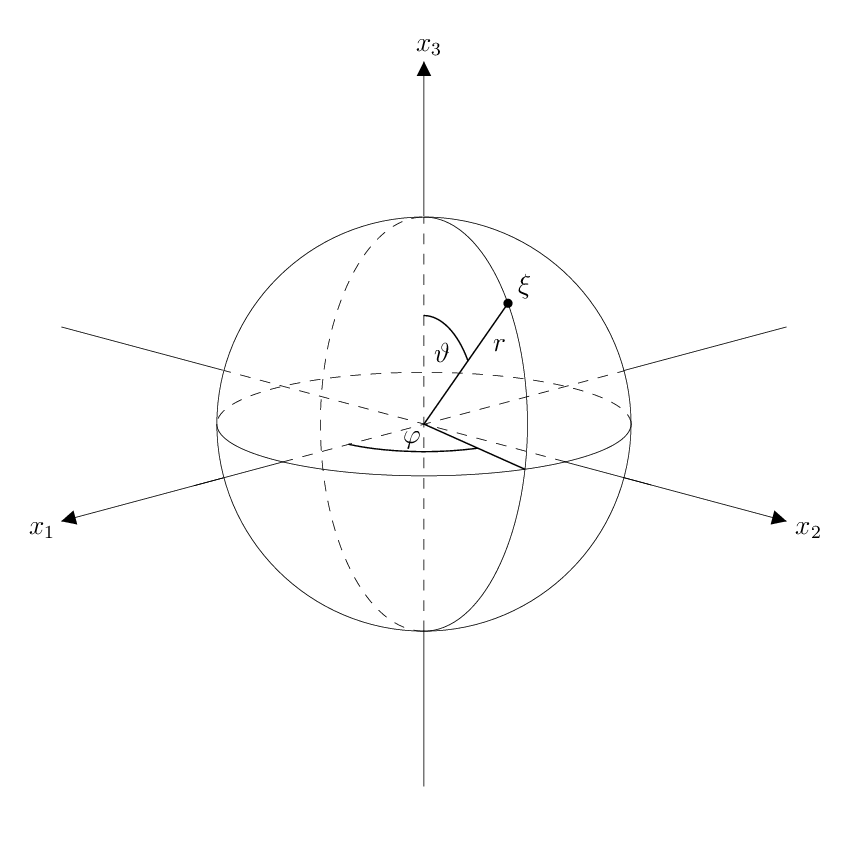
\includegraphics[width=.4\textwidth]{Figures/sphere.png}
%        \end{figure}
%        \end{ex}
%        
%        \begin{ex}{The Hyperboloids}{hyperboloids}
%        Consider a family of surfaces given by the level surfaces of
%        \[
%        f(x,y,z)=x^2+y^2-z^2.
%        \]
%        \begin{itemize}
%            \item If we take $c=0$ and set
%            \[
%            x^2+y^2-z^2=0.
%            \]
%            then we find the 0 level surface. In this case, we can do a bit of work to find
%            \[
%            z=\pm \sqrt{x^2+y^2}.
%            \]
%            Notice, if we pick any value for $z$, that we get a circle at that level!  When $z=0$, we get a single point.  It turns out that we get the \emph{(double) cone} surface which looks like
%            \begin{figure}[H]
%                \centering
%             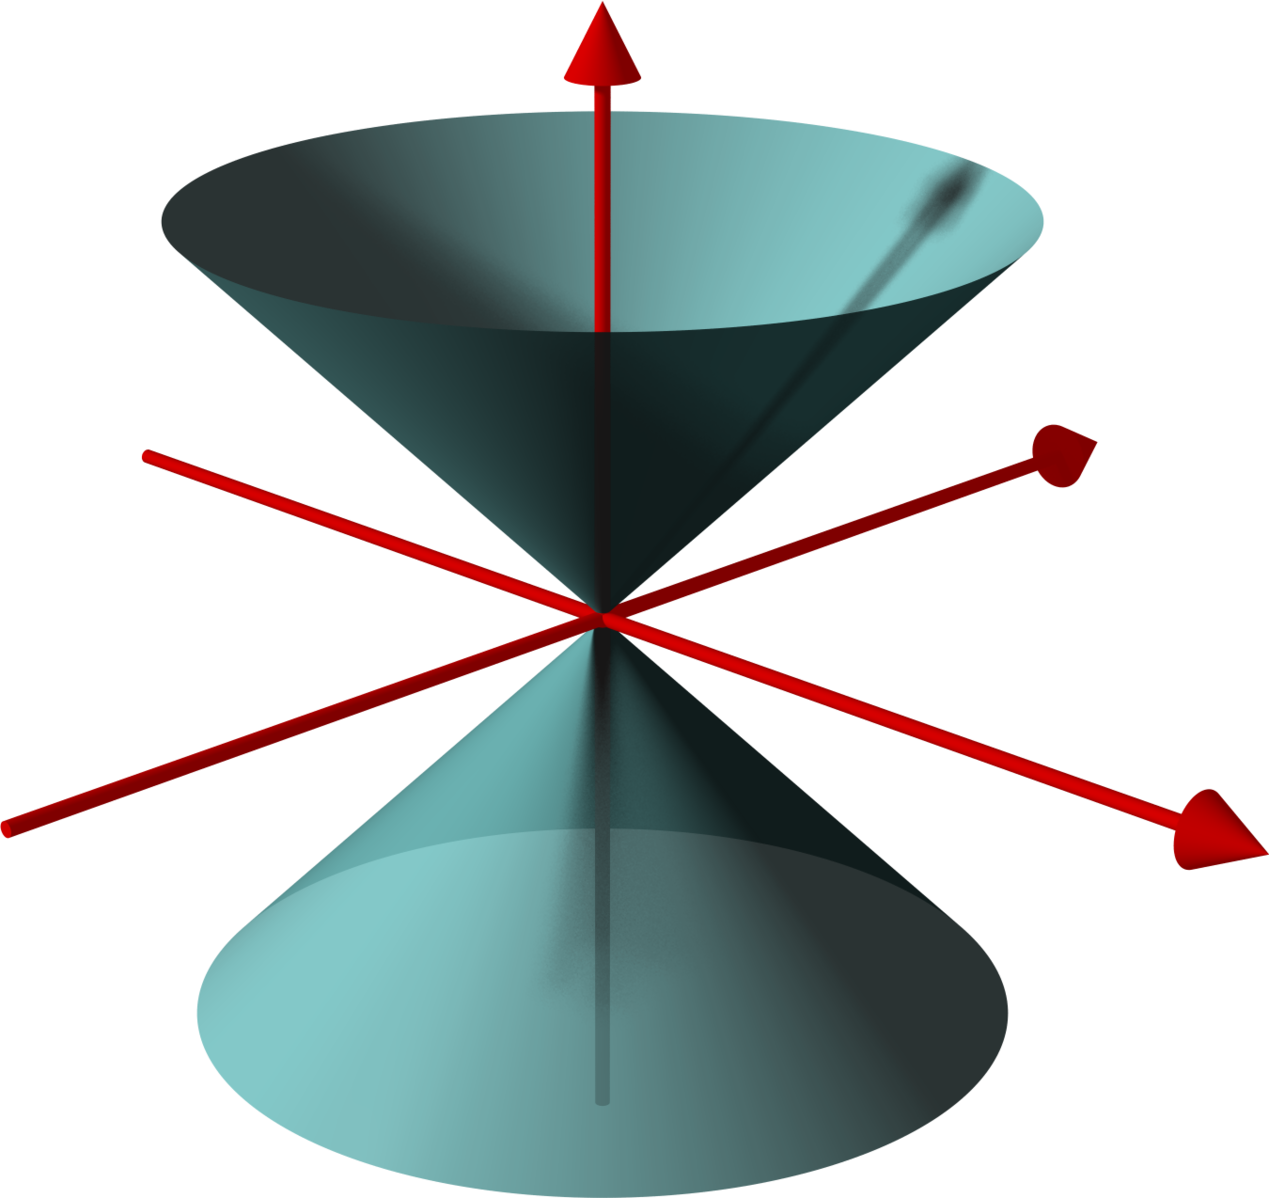
\includegraphics[width=.4\textwidth]{Figures/cone_surface.png}
%            \end{figure}
%            
%            \item If we take $c=1$ and set
%            \[
%            x^2+y^2-z^2=1
%            \]
%            we get the \emph{hyperboloid of one sheet}.  This looks like
%            \begin{figure}[H]
%                \centering
%                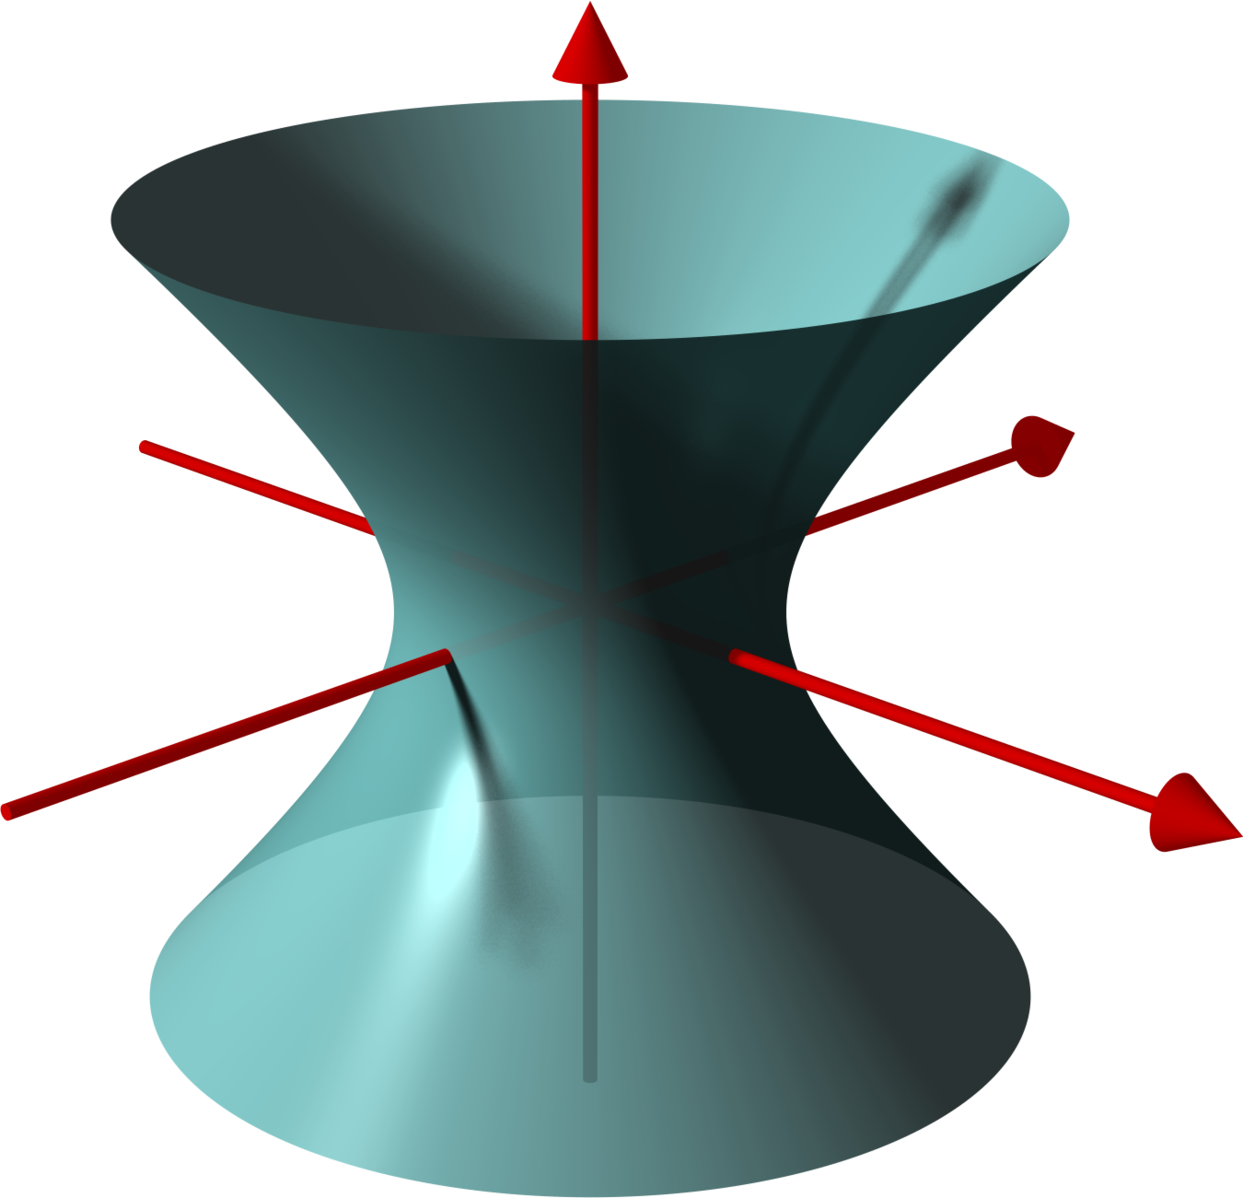
\includegraphics[width=.4\textwidth]{Figures/hyperboloid_1_sheet.png}
%            \end{figure}
%            
%            \item If we take $c=-1$ and set
%            \[
%            x^2+y^2-z^2=-1
%            \]
%            we get the \emph{hyperboloid of two sheets}.  This looks like
%            \begin{figure}[H]
%                \centering
%                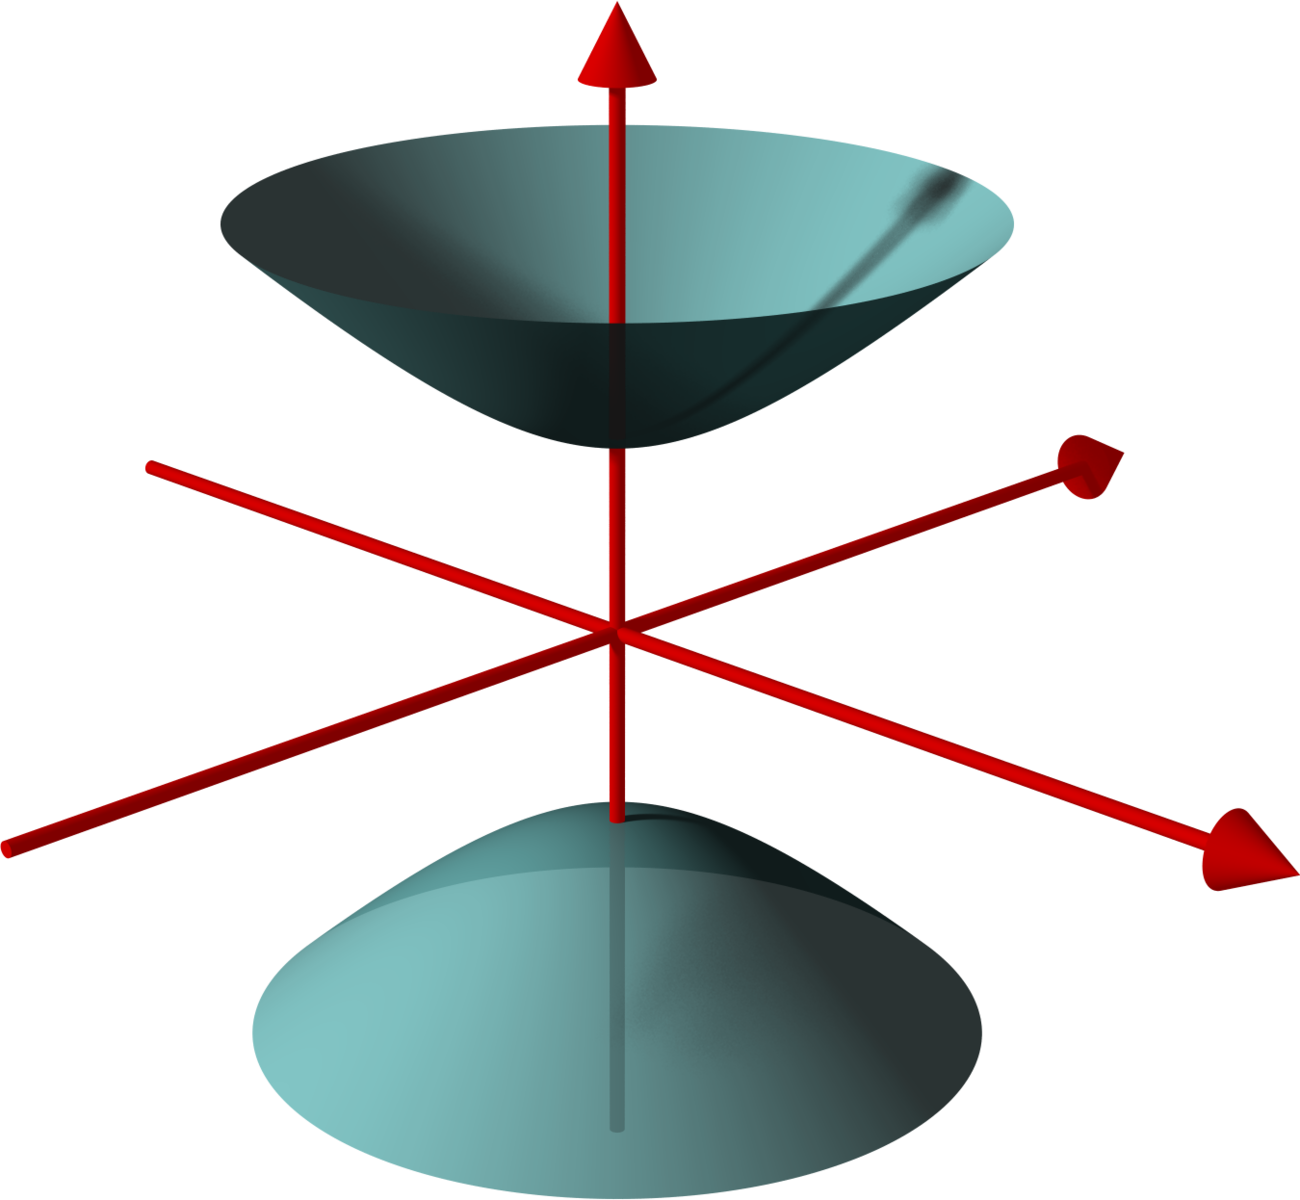
\includegraphics[width=.4\textwidth]{Figures/hyperboloid_2_sheet.png}
%            \end{figure}
%        \end{itemize}
%        \end{ex}
%        
%        \begin{ex}{The Torus}{torus}
%        For this example, I will choose specific nice numbers, but this is a yet another case of a level surface.  Take
%        \[
%        \left(5-\sqrt{x^2+y^2}\right)^2+z^2=2.
%        \]
%        This gives us the \emph{torus} with inner radius (the radius from the center of the donut hole to the center of the tube) $5=R$ and tube radius $2=r$. This looks like
%        \begin{figure}[H]
%            \centering
%            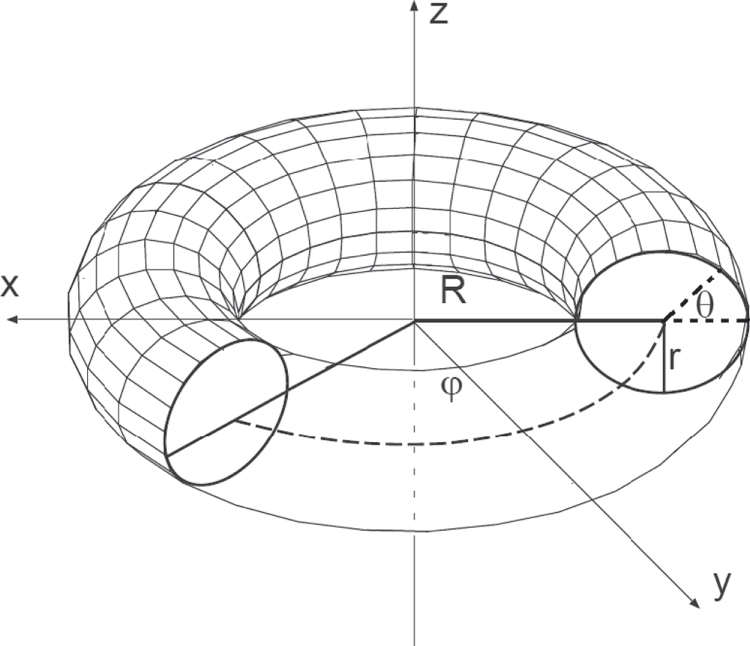
\includegraphics[width=.4\textwidth]{Figures/torus.png}
%        \end{figure}
%        \end{ex}
%        
%        
%        We have given ourselves ways of understanding the scalar functions and curves, but still need to develop a manner to understand vector fields.  We will not only need to understand vector fields in their own right, but we will need them in order to investigate how the scalar fields change from point to point.  Roughly speaking, the ``derivative" of a scalar field will be a vector field.
%        
%        \section{Vector Fields}
%        
%        A vector field is a function that inputs a vector and outputs a vector. Specifically, we can write
%        \[
%        \mathbf{v}(x,y,z)=(f_1(x,y,z),f_2(x,y,z),f_3(x,y,z))=\begin{bmatrix} f_1(x,y,z)\\ f_2(x,y,z) \\ f_3(x,y,z)\end{bmatrix}.
%        \]
%        Notice the differences and similarities between vector fields, scalar fields, and curves.  Just as before, it will be nice to visualize many vector fields in the $xy$-plane to avoid drawing in 3-dimensions. Of course, we can use technology to make nice plots in space.
%        
%        Intuitively, a vector field is an assignment of a vector at each point in space.  To match this intuition we tend to just draw a collection of arrows in space.
%        
%        \begin{ex}{Eastward Wind}{east_wind}
%        Consider the vector field
%        \[
%        \mathbf{v}\colon \R^2 \to \R^2
%        \]
%        given by
%        \[
%        \mathbf{v}(x,y)=(1,0).
%        \]
%        At each point $(x,y)$, we are assigning a vector that points a distance 1 in the $x$-direction. See the following figure.
%        \begin{figure}[H]
%            \centering
%            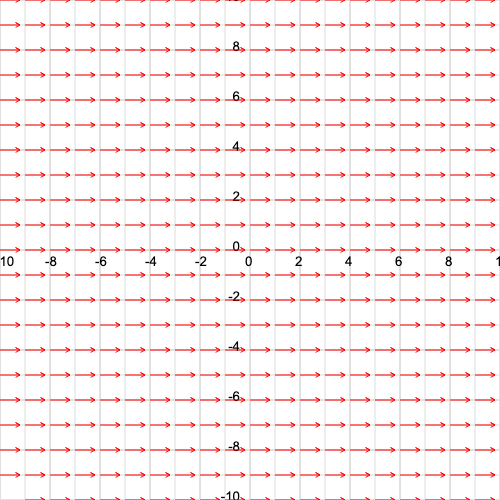
\includegraphics[width=.6\textwidth]{Figures/wind_field.png}
%        \end{figure}
%        \end{ex}
%        
%        \begin{ex}{Line Source}{line_source}
%        Consider the vector field in the plane given by
%        \[
%        \mathbf{v}(x,y)=(x+y,x+y).
%        \]
%        See the following figure.
%        \begin{figure}[H]
%            \centering
%            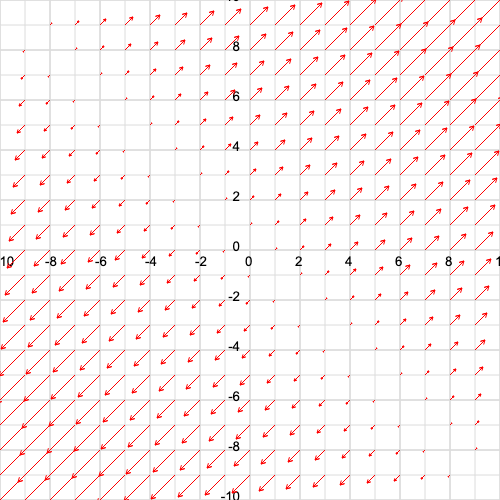
\includegraphics[width=.6\textwidth]{Figures/v_field_1.png}
%        \end{figure}
%        \end{ex}
%        
%        \begin{ex}{Whirlpool}{whirlpool}
%        Consider the vector field in the plane given by
%        \[
%        \mathbf{v}(x,y)=(y,-x).
%        \]
%        See the following figure.
%        \begin{figure}[H]
%            \centering
%            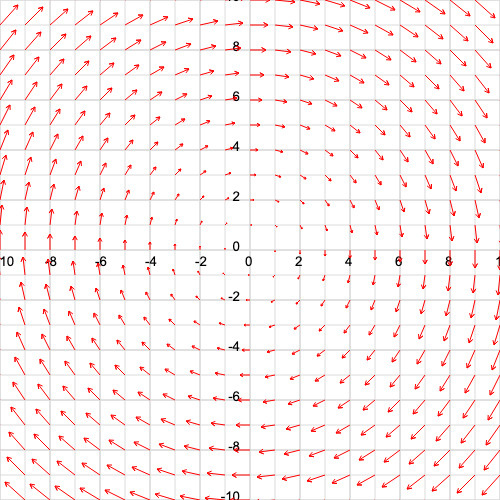
\includegraphics[width=.6\textwidth]{Figures/v_field_3.png}
%        \end{figure}
%        \end{ex}
%        
%%    \chapter{Calculus with Multivariate Functions}
%        
%        \section{Differentiation of fields}
%        One may now wonder where the calculus comes in.  We are almost there, but we should know what it means intuitively to use the calculus tools with these more general fields.
%        
%        Curves will prove to be a great tool in the analysis of these scalar fields.  We will also need to understand how vectors transform from point to point which will require us to recall the knowledge we gained on linear transformations.
%        
%        Roughly speaking, we will have:
%        \begin{itemize}
%            \item \textbf{Curves:} Derivatives of curves $\gamma(t)$ are vectors. Specifically, we have already seen the tangent vector $\gamma'(t)$ and acceleration vector $\gamma''(t)$.
%            \item \textbf{Scalar Fields:} Derivatives of scalar fields $f(x,y,z)$ will depend on which input of the function we change.  We can collect the partial derivatives corresponding to finding derivatives in one input into a vector called the \emph{gradient}.
%            \item \textbf{Vector Fields:} Derivatives of vector fields $\mathbf{v}(x,y,z)$ will require us to see how each component of $\mathbf{v}$ changes based on how each individual input changes.  In this case, this collection of derivatives will be put into a matrix known as the \emph{total derivative}.
%        \end{itemize}
%        
%        \begin{remark}
%        The important notion that we need to understand is the following.
%        
%        \emph{The derivative of a function at a point is the best linear approximation to the function.} 
%        
%        Based on this wording, it is intuitive to imagine derivatives as vectors or matrices.
%        \end{remark}
%        
%        \section{Functions of Fields}
%        In our world, we often care about combining different fields together.  For example, we can take the electric field created by a single charged particle and add this field to another field created by a different charged particle. What I mean, is we can write
%        \[
%        \mathbf{v}(x,y,z)+\mathbf{u}(x,y,z)
%        \]
%        and make sense of this.  Just as we did with vectors, we add the components together! That is if we have
%        \begin{align*}
%        \mathbf{v}(x,y,z)&=(f_1(x,y,z),f_2(x,y,z),f_3(x,y,z))\\ \mathbf{u}(x,y,z)&=(g_1(x,y,z),g_2(x,y,z),g_3(x,y,z)),
%        \end{align*}
%        then
%        \[
%        \mathbf{v}(x,y,z)+\mathbf{u}(x,y,z)=(f_1+g_1,f_2+g_2,f_3+g_3).
%        \]
%        Intuitively, this just adds together the vectors at each point!
%        
%        \begin{ex}{Addition of vector fields}{add_vect_fields}
%        Consider the following vector fields
%        \begin{align*}
%            \mathbf{v}(x,y)&=(x,x)\\
%            \mathbf{u}(x,y)&=(y,y).
%        \end{align*}
%        These look like:
%        \begin{figure}[H]
%            \centering
%            \begin{subfigure}[h]{.45\textwidth}
%            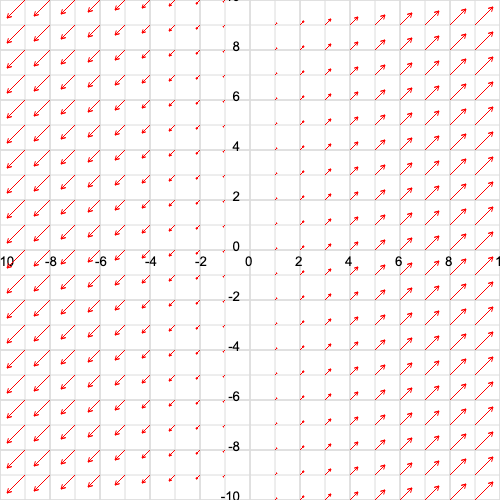
\includegraphics[width=\textwidth]{Figures/vec_v.png}
%            \caption{Vector field $\mathbf{v}$.}
%            \end{subfigure}
%            ~
%            \begin{subfigure}[h]{.45\textwidth}
%            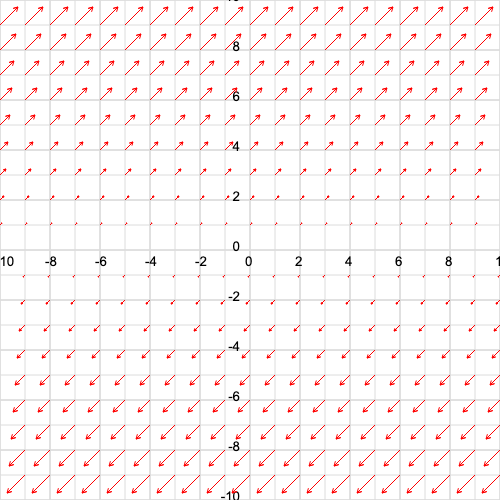
\includegraphics[width=\textwidth]{Figures/vec_u.png}
%            \caption{Vector field $\mathbf{u}$.}
%            \end{subfigure}
%        \end{figure}
%        Adding these results in the field
%        \begin{figure}[h]
%            \centering
%            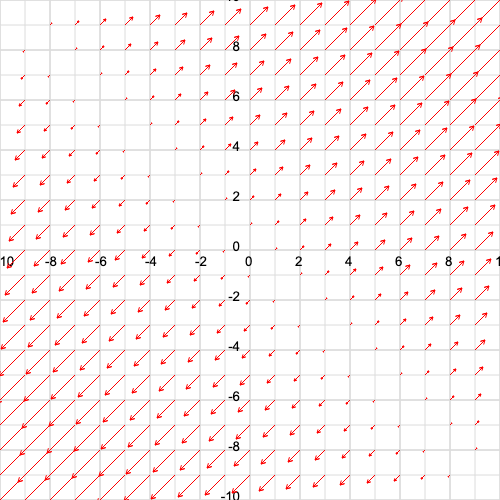
\includegraphics[width=.45\textwidth]{Figures/v_field_1.png}
%            \caption{Caption}
%            \label{fig:my_label}
%        \end{figure}
%        \end{ex}
%        
%        \begin{remark}
%        If we do this all for vector fields, we can take curves and scalar fields as special cases.
%        \begin{itemize}
%            \item Adding together scalar fields is the same as adding functions.  They just have more inputs to think about!
%            \item Adding together curves is done in the same componentwise manner that we have shown here for vector fields.
%        \end{itemize}
%        \end{remark}
%        
%        We can also scale a field by a real number.  This will stretch vectors at each point.
%        
%        \begin{ex}{Scaling of Vector Fields}{scale_vect_field}
%        Just take the vector field
%        \[
%        \mathbf{v}(x,y,z)=(f_1(x,y,z),f_2(x,y,z),f_3(x,y,z))
%        \]
%        then we can take
%        \[
%        \lambda \mathbf{v}=(\lambda f_1, \lambda f_2, \lambda f_3).
%        \]
%        \end{ex}
%        
%        \begin{remark}
%        There is many reasons why the above is important.  It seems our physical world plays nicely with the above concept, for one.
%        
%        One thing we can actually do, and will do a bit later, is find that there are two main types of vector fields in $\R^3$.  These will be the curl fields and divergence fields!  This is important in electromagnetism.
%        \end{remark}
%        
%        When we were working with complex numbers, we considered integrating a complex function $f(z)$ over a contour $\gamma(t)$ from $t=a$ to $t=b$.  This involved computing
%        \[
%        \int_\gamma f(\gamma)d\gamma = \int_a^b f(\gamma(t))\gamma'(t)dt.
%        \]
%        I introduced this concept since it appears in the context of multivariate functions.  However, in the multivariate case, we needed some more tools.
%        
%        Now, the idea is as follows.  We will be given a scalar field, $f(x,y,z)$ or a vector field $\mathbf{F}(x,y,z)$ and a curve $\gamma(t)$.  
%        
%        \section{Line integrals of scalar fields}
%        For the purpose of visualization, we will look at scalar fields of two variables and curves in the plane.  Our set up will have $f(x,y)$ and $\gamma(t)$ over the time $t=a$ to $t=b$.
%        
%        We want to understand the following:
%        \[
%        \int_\gamma f(\gamma)d\gamma \coloneqq \int_a^b f(\gamma(t))\|\gamma'(t)\|dt.
%        \]
%        Intuitively speaking, this integral finds the area under the curve $\gamma$ along the graph of $f$.  This is analogous to what we did in one dimension! See the following figure.
%        \begin{figure}[H]
%            \centering
%            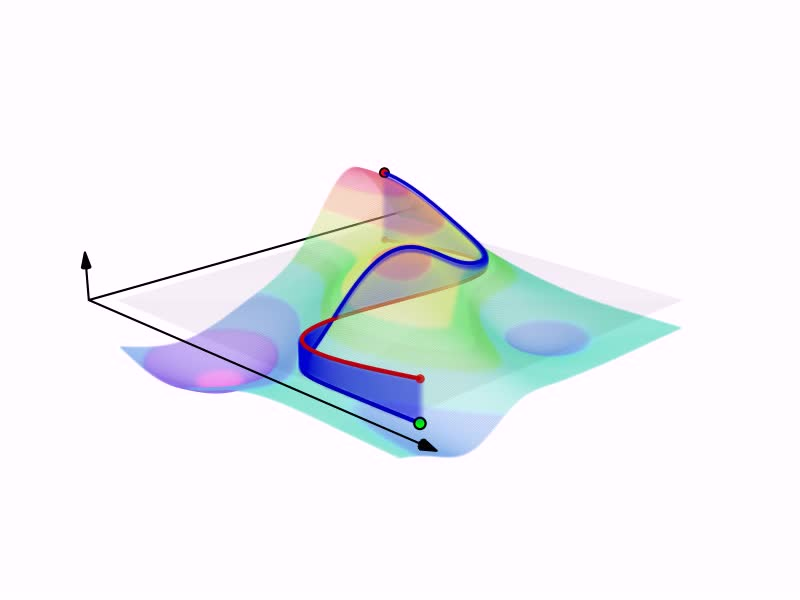
\includegraphics[width=.5\textwidth]{Figures/Line_integral_of_scalar_field.jpg}
%        \end{figure}
%        
%        \begin{ex}{Length of a curve}{length_of_curve}
%        Let $f(x,y,z)=1$ and $\gamma(t)$ be a curve over $t=a$ to $t=b$.  Then the line integral
%        \[
%        \int_\gamma f(\gamma)d\gamma = \int_a^b \|\gamma'(t)\|dt
%        \]
%        is known as the \emph{length} (sometimes \emph{arclength} of the curve $\gamma$.
%        \end{ex}
%        
%        \begin{ex}{Line Integral on a Paraboloid}{line_int_parabooid}
%        Consider the function $f(x,y)=x^2+y^2$ and $\gamma(t)=(t,t)$ over $t=0$ to $t=1$.  Then the line integral
%        \[
%        \int_\gamma f(\gamma)d\gamma = \int_0^1 f(\gamma(t))\|\gamma'(t)\|dt.
%        \]
%        We have
%        \begin{itemize}
%            \item $f(\gamma(t))=t^2+t^2=2t^2.$
%            \item $\|\gamma'(t)\|=\|(1,1)\|=\sqrt{2}.$
%        \end{itemize}
%        So we have
%        \[
%        \int_\gamma f(\gamma)d\gamma = \int_0^1 2\sqrt{2}t^2dt.
%        \]
%        This evaluates to $\frac{2\sqrt{2}}{3}$.
%        \end{ex}
%        
%        \begin{exercise}
%        Integrate $f(x,y)=x+y$ along the curve $\gamma(t)=(t,0)$ from $t=0$ to $t=1$. What do you notice about this? Can we tie this to one-dimensional integration?
%        \end{exercise}
%        
%        \section{Line integrals of vector fields}
%        
%        There is also a type of line integral that works alongside vector fields.  Roughly, the idea is to add up how much a vector field is pointing along the curve throughout the length of the curve.  
%        
%        Here we are given $\mathbf{F}(x,y,z)$ is a vector field, $\gamma(t)$ is a curve over the time $t=a$ to $t=b$.  Then we can write
%        \[
%        \int_\gamma \mathbf{F}(\gamma)\cdot d\gamma =\int_a^b \mathbf{F}(\gamma(t))\cdot \gamma'(t) dt.
%        \]
%        
%        \begin{ex}{Work Done on a Particle}{work_on_particle}
%        The work done on a particle (or change in energy) is written as a line integral of this form.  
%        
%        Take for example, $\mathbf{F}(x,y)=(2x,3y)$ and $\gamma(t)=(t,t^2)$ over the time $t=0$ to $t=1$.  Then
%        \begin{align*}
%        \int_\gamma \mathbf{F}(\gamma)\cdot d\gamma &= \int_0^1 \mathbf{F}(t,t^2)\cdot (t,t^2)dt\\
%        &= \int_0^1 (2t,2t^2)\cdot(t,t^2)dt\\
%        &=\int_0^1 2t^2+2t^4dt.
%        \end{align*}
%        Which I'll leave to you to evaluate if you'd like.
%        \end{ex}
%        
%        \begin{remark}
%        This notion is extremely important in defining something called the \emph{potential} of a vector field.  This will show up in electrodynamics.
%        
%        If the force in the example above is \emph{conservative}, we will have a potential.  This will correspond nicely to the vector field having no \emph{curl}.
%        \end{remark}
%        
%        \section{Derivatives}
%        Having done some integral calculus, it's time to head back to differential calculus.  We should say the following. This is far more abstract than we need, but it is an important realization.  
%        
%        \begin{df}{The Derivative}{derivative}
%        Given a function $f\colon \R^n \to \R^m$, the \textbf{derivative of $f$ at the point $\mathbf{x}_0$} is the best \emph{linear approximation} to $f$ at the point $\mathbf{x}_0$.
%        
%        What this means is the following: If we zoom in to the point $\mathbf{x}_0$ and see what $f$ does in this region, we'll notice that $f$ is approximately a linear transformation.
%        \end{df}
%        
%        Now, let us review the one-dimensional derivative that we are familiar with.
%        
%        \begin{df}{Derivative on $\R$}{der_on_R}
%        Given $f\colon \R \to \R$, we define the \textbf{derivative $f'$ of $f$ at the point $x_0$} by
%        \[
%        f'(x_0)\coloneqq \lim_{\delta \to 0} \frac{f(x_0+\delta)-f(x_0)}{\delta}.
%        \]
%        This value $f'(x_0)$ is a number, and moreover is a $1\times 1$-matrix!  We often hide this idea at first.
%        \end{df}
%        
%        It's a bit silly to say $f'(x_0)$ is a $1\times 1$-matrix, but in the end it will help us to remember this.
%        
%        \subsubsection{Derivatives of scalar fields}
%        We can investigate functions of multiple variables in more ways than the single variable case.  Let us start with scalar fields.
%        
%        \begin{df}{Partial Derivatives}{partial_derivs}
%        Let $f\colon \R^3 \to \R$ be a scalar field.  Then we can consider derivatives with respect to changing each input.  For example, we define the \textbf{partial derivative with respect to $x$} \textbf{at the point $(x_0,y_0,z_0)$}, denoted $\frac{\partial f}{\partial x}$, and put
%        \[
%        \frac{\partial f}{\partial x}(x_0,y_0,z_0)\coloneqq \lim_{\delta \to 0} \frac{f(x_0+\delta,y_0,z_0)-f(x_0,y_0,z_0)}{\delta}
%        \]
%        \end{df}
%        
%        \begin{remark}
%        For partial derivatives, all but one variable are being held constant.  So, when you are computing these, be sure to treat the proper variables as constant when necessary.
%        \end{remark}
%        
%        \begin{exercise}
%        Define $\frac{\partial f}{\partial y}$ and $\frac{\partial f}{\partial z}$ in a similar way to the above definition.
%        \end{exercise}
%        
%        \begin{exercise}
%        Compute $\partialx$, $\partialy$, and $\partialz$ for the function 
%        \[
%        f(x,y,z)=\sin(xyz)+x+2y^2+3x^2z.
%        \]
%        \end{exercise}
%        
%        It turns out that collecting the partial derivatives as a vector is the best linear approximation to a scalar function.  We call this vector the gradient vector.
%        
%        \begin{df}{The Gradient}{gradient}
%        Given a scalar field $f(x,y,z)$, the \textbf{gradient of $f$ at the point $(x_0,y_0,z_0)$}, denoted $\nabla f(x_0,y_0,z_0)$ is given by
%        \[
%        \nabla f(x_0,y_0,z_0)=\begin{bmatrix} \partialx(x_0,y_0,z_0)\\ \partialy(x_0,y_0,z_0)\\ \partialz(x_0,y_0,z_0)\end{bmatrix}.
%        \]
%        \end{df}
%        
%        \begin{exercise}
%        Compute the gradient for the function
%        \[
%        f(x,y,z)=\sin(xyz)+x+2y^2+3x^2z.
%        \]
%        \end{exercise}
%        
%        \subsubsection{Properties of partial derivatives and the gradient}
%        
%        As with the one-dimensional derivative, we have some properties that will be helpful.\\
%        
%        \noindent\textbf{Partial Derivatives:}
%        \begin{enumerate}[(i)]
%            \item \textbf{Sum Rule:} Given $f(x,y,z)$ and $g(x,y,z)$, we have that
%            \[
%            \frac{\partial}{\partial x} (f(x,y,z)+g(x,y,z))=\partialx + \frac{\partial g}{\partial x}.
%            \]
%            Of course, this holds for any partial derivative.
%            \item \textbf{Constant Multiple:} Given $\lambda \in \R$ and $f(x,y,z)$, we have that
%            \[
%            \frac{\partial}{\partial x}(\lambda f(x,y,z))=\lambda \partialx.
%            \]
%            Again, this holds for any partial derivative.
%            \item \textbf{Product Rule:} Given $f(x,y,z)$ and $g(x,y,z)$ we have that
%            \[
%            \frac{\partial }{\partial x}(f(x,y,z)g(x,y,z))=\partialx g + f \frac{\partial g}{\partial x}.
%            \]
%            Ths holds for all partial derivatives.
%        \end{enumerate}
%        
%        \begin{remark}
%        The chain rule will show up eventually, but not yet.  As for the quotient rule, this also holds, but I don't show it here.
%        \end{remark}
%        
%        \noindent\textbf{The Gradient:}
%        \begin{enumerate}[(i)]
%            \item \textbf{Sum Rule:} Given $f(x,y,z)$ and $g(x,y,z)$, we have that
%            \[
%            \nabla(f(x,y,z)+g(x,y,z))=\nabla f(x,y,z)+\nabla g(x,y,z).
%            \]
%            \item \textbf{Constant Multiple:} Given $\lambda \in \R$ and $f(x,y,z)$, we have that
%            \[
%            \nabla(\lambda f(x,y,z))=\lambda \nabla f(x,y,z).
%            \]
%            \item \textbf{Product Rule:} Given $f(x,y,z)$ and $g(x,y,z)$ we have that
%            \[
%            \nabla(f(x,y,z)g(x,y,z))=(\nabla f(x,y,z))g(x,y,z)+f(x,y,z)(\nabla g(x,y,z))
%            \]
%            
%        \end{enumerate}
%        
%        We've learned how to compute partial derivatives and the gradient, but what are they really telling us? Remember that the derivative $\frac{d}{dx}$ of a function $f(x)$ tells us the rate of change of $f$ as we move in the $x$-direction.  This is very similar to what $\frac{\partial}{\partial x}$ tells us about a function $f(x,y,z)$.  So we can say the following.
%        \begin{itemize}
%            \item $\frac{\partial f}{\partial x}$ tells us how $f$ changes as we move in the $x$-direction.
%            \item $\frac{\partial f}{\partial y}$ tells us how $f$ changes as we move in the $y$-direction.
%            \item $\frac{\partial f}{\partial z}$ tells us how $f$ changes as we move in the $z$-direction.
%        \end{itemize}
%        
%        We can put these together into the gradient $\nabla f$ and know how $f$ changes in each possible direction. Let's see how the gradient acts then. 
%        
%        \begin{ex}{Gradients on the Paraboloid}
%        Let us start with $f(x,y)=x^2+y^2$.  Then
%        \[
%        \nabla f(x,y) = (2x,2y).
%        \]
%        Let us plot the level curves of this surface.
%        \begin{figure}[H]
%            \centering
%            \begin{subfigure}[h]{.45\textwidth}
%            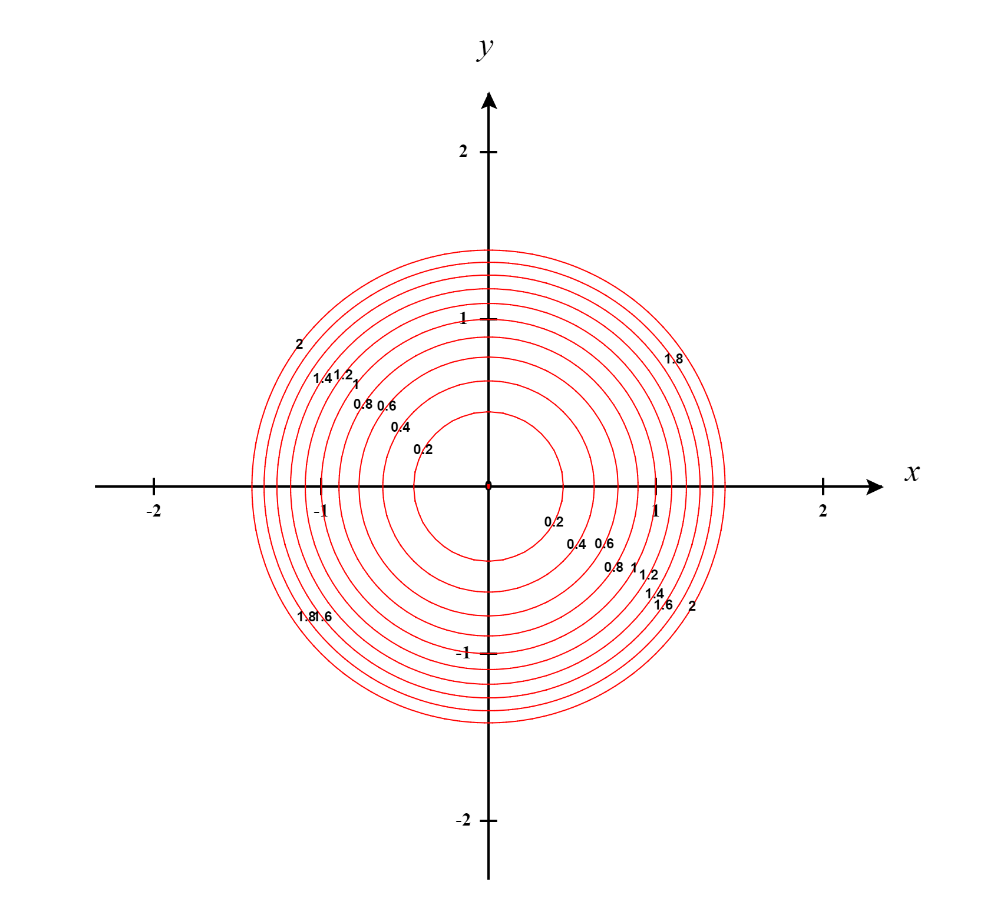
\includegraphics[width=\textwidth]{Figures/level_curves_gradient.png}
%            \caption{Level curves of $f(x,y)$.}
%            \end{subfigure}
%            ~
%            \begin{subfigure}[h]{.45\textwidth}
%            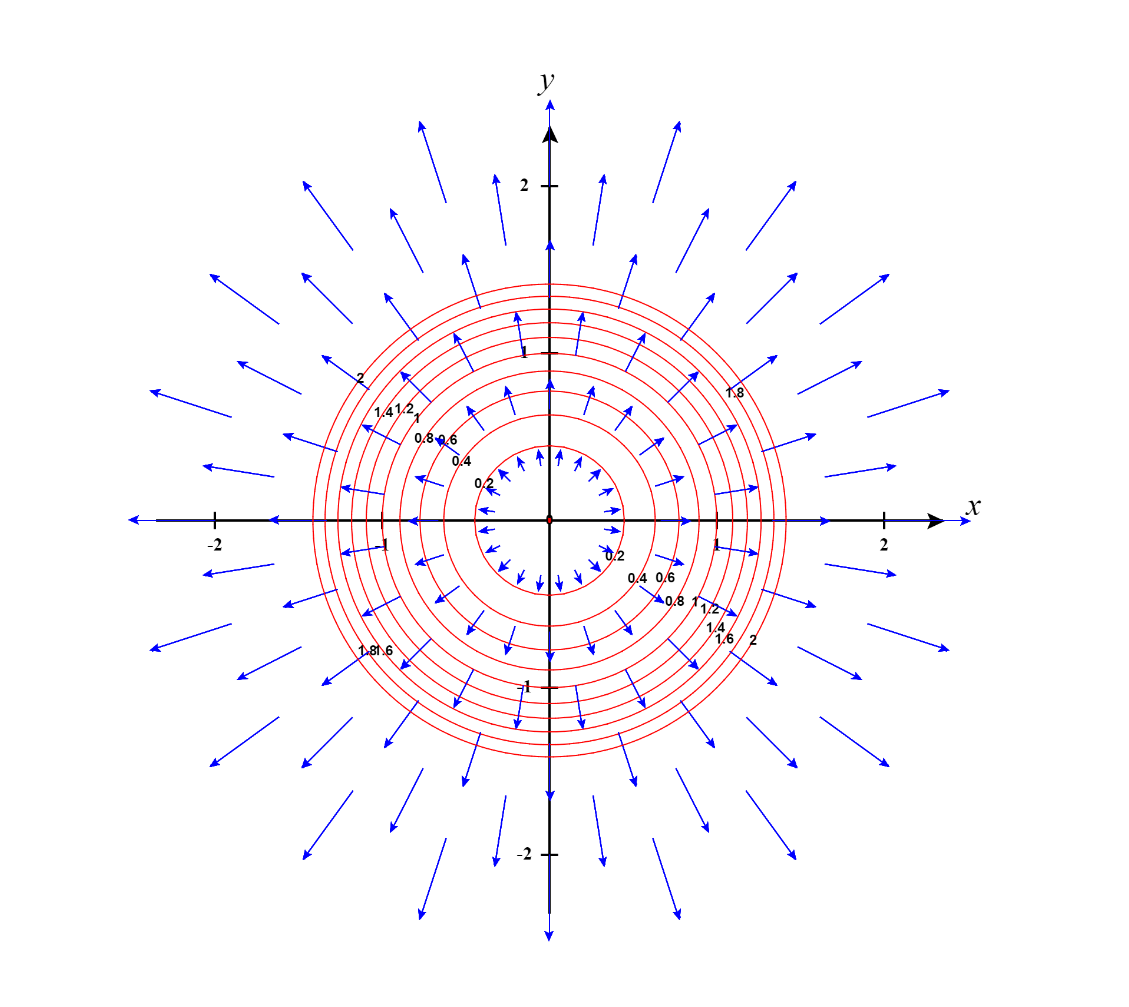
\includegraphics[width=\textwidth]{Figures/level_curves_gradient_vectors.png}
%            \caption{Gradient vectors shown in blue.}
%            \end{subfigure}
%        \end{figure}
%        \begin{itemize}
%            \item Notice that the gradient vectors point in a direction perpendicular to the level curves and the length corresponds to how close the nearest level curve is.
%            \item The gradient is zero at the bottom of this surface.  
%        \end{itemize}
%        \end{ex}
%        
%        \begin{prop}{Gradient Points Uphill}{gradient_prop}
%        The gradient $\nabla f(x,y,z)$ is the vector that points in the direction of greatest increase for a function $f(x,y,z)$.
%        \end{prop}
%        
%        How about second partial derivatives? What can we say here. We have each of the following for a function $f(x,y)$:
%        \begin{itemize}
%            \item $\frac{\partial^2 f}{\partial x^2}$
%            \item $\frac{\partial^2 f}{\partial y^2}$
%            \item $\frac{\partial}{\partial y}\frac{\partial f}{\partial x}$
%            \item $\frac{\partial}{\partial x}\frac{\partial f}{\partial y}$
%        \end{itemize}
%        
%        Recall what $\frac{d^2 f}{dx^2}$ meant for a function $f(x)$.  This told us how $f$ was curving (or what concavity $f$ had). The story is similar for these partial derivatives.
%        
%        \begin{itemize}
%            \item $\frac{\partial^2 f}{\partial x^2}$ tells us about the concavity (or curvature) of $f$ as we move in the $x$ direction.
%            \item $\frac{\partial^2 f}{\partial y^2}$ tells us about the concavity (or curvature) of $f$ as we move in the $y$ direction.
%            \item We actually have that $\frac{\partial}{\partial y}\frac{\partial f}{\partial x}=\frac{\partial}{\partial x}\frac{\partial f}{\partial y}$.  This interpretation is a bit hard to deal with.  Let's not worry too much about it.
%        \end{itemize}
%        
%        \begin{prop}{Partial Derivatives Commute}{partials_commute}
%        We have that
%        \[
%        \frac{\partial}{\partial y}\frac{\partial f}{\partial x}=\frac{\partial}{\partial x}\frac{\partial f}{\partial y}.
%        \]
%        Moreover, for functions of more variables, we can say that the order we take derivatives does not matter.
%        \end{prop}
%        
%        \begin{exercise}
%        Given $f(x,y)=x^2+y^2$, compute
%        \[
%        \frac{\partial^2 f}{\partial x^2}, ~ \frac{\partial^2 f}{\partial y^2}, ~ \frac{\partial}{\partial y}\frac{\partial f}{\partial x},~ \frac{\partial}{\partial x}\frac{\partial f}{\partial y}.
%        \]
%        What can we say about the curvature of $f$ in the two directions? Does this make sense?
%        \end{exercise}
%        
%        \section{Optimization}
%        In single variable calculus, we optimized functions $f(x)$ by finding the point $x_0$ where 
%        \[
%        f'(x_0)=0.
%        \]
%        We called this a \emph{critical point}. We found if this optimizer $x_0$ was a maximizer or minimizer by checking the sign of second derivative $f''(x_0)$. We had
%        \begin{align*}
%            \textrm{Maximum: }& f''(x_0)<0\\
%            \textrm{Minimum: }& f''(x_0)>0.
%        \end{align*}
%        
%        In higher dimensions, this idea works similarly. We just have more to check. 
%        
%        \begin{df}{Stationary Points}{stationary_points}
%        Given a function $f(x,y)$, we call a point $(x_0,y_0)$ a \textbf{stationary point} if 
%        \[
%        \nabla f(x_0,y_0) = \mathbf{0}.
%        \]
%        \end{df}
%        
%        As before, we will use second derivatives to find out whether this is a maximum or a minimum.
%        
%        \begin{prop}{Maximizers and Minimizers}{max_min}
%        A stationary point $(x_0,y_0)$ is a 
%        \begin{align*}
%            \textrm{Maximizer if~ }& \frac{\partial^2 f}{\partial x^2} <0 \textrm{ ~and~ } \frac{\partial^2 f}{\partial y^2}<0,\\
%            \textrm{Minimizer if~ }& \frac{\partial^2 f}{\partial x^2} >0 \textrm{ ~and~ } \frac{\partial^2 f}{\partial y^2}>0,\\
%            \textrm{Saddle if otherwise.}
%        \end{align*}
%        \end{prop}
%        
%        \begin{exercise}
%        Let
%        \[
%        f(x,y) = \frac{xy}{e^{x^2+y^2}}.
%        \]
%        \begin{enumerate}[(a)]
%            \item Find all stationary points for $f$.
%            \item Determine whether these points are minimizers or maximizers.
%        \end{enumerate}
%        \end{exercise}
%        
%        \begin{exercise}
%        Show that $f(x,y)=xy$ has a saddle point at $(0,0)$.
%        \end{exercise}
%        
%        \subsubsection{Lagrange Multipliers}
%        Often times we are given a situation that we wish to find an optimum solution to, but we are somehow constrained.  A biological example would be fixing a given volume for a red blood cell, and finding the optimum shape so that oxygen diffusion is maximized.  A physical example would be finding the fastest path between two points when moving through a medium with varying viscosity.
%        
%        The idea is relatively tame. We are given the function to optimize
%        \[
%        f(x,y,z)
%        \]
%        and the constraining function
%        \[
%        g(x,y,z)=k.
%        \]
%        Then we must solve the equation
%        \[
%        \nabla f(x,y,z) = \lambda \nabla g (x,y,z)
%        \]
%        where $\lambda$ is called the \textbf{Lagrange multiplier}. Let's work through an example of solving this.
%        
%        \begin{ex}{Largest Box}{largest_box}
%        Let's find the dimensions of the box with the largest volume if the total surface area is $64 cm^2$.  We must determine our function to optimize, which is the volume function
%        \[
%        V(x,y,z) = xyz.
%        \]
%        Our constraint is the surface area function $A(x,y,z)$ must be
%        \[
%        g(x,y,z)=2xy+2xz+2yz=64,
%        \]
%        which we will simplify as
%        \[
%        xy+xz+yz = 32.
%        \]
%        \begin{enumerate}
%            \item We first take
%            \[
%            \nabla f(x,y,z) = \begin{bmatrix} yz \\ xz \\ xy \end{bmatrix}
%            \]
%            and
%            \[
%            \nabla g(x,y,z) = \begin{bmatrix} 2y+2z \\ 2x+2z \\ 2x+2y\end{bmatrix}.
%            \]
%            \item This gives us four equations to solve. Three are from the equation $\nabla f(x,y,z) =\nabla g(x,y,z)$
%            \begin{align}
%                yz &= \lambda (y+z)\\
%                xz &= \lambda (x+z)\\
%                xy &= \lambda (x+y),
%            \end{align}
%            and one is from the constraint $g(x,y,z)=64$
%            \[
%            xy+xz+yz = 32.
%            \]
%            \item Working through solving these can be nontrivial.  In this case, we can do the following: Multiply (1) by $x$, (2) by $y$, and $(3)$ by $z$.  Which gives us
%            \begin{align*}
%                xyz &= \lambda x(y+z)\\
%                xyz &= \lambda y(x+z)\\
%                xyz &= \lambda z(x+y)
%            \end{align*}
%            Now we can set the first two equal to find
%            \[
%            \lambda x(y+z)=\lambda y(x+z)
%            \]
%            which simplifies to 
%            \[
%            \lambda (xz-yz)=0
%            \]
%            meaning that $\lambda =0$ or $xz=yz$. Note that $\lambda =0$ is not possible since that will end up giving us zero surface area and we won't satisfy the constraint.
%            
%            Now $xz-yz=0$ means that $x=y$, which we can substitute back into the equations later. 
%            
%            We can set the last two equal to find
%            \[
%            \lambda y (x+z)=\lambda z(x+y)
%            \]
%            which with similar work tells us $z=y$.  So now we make note of $x=y$ and we have $x=y=z$.  
%            
%            So now we use the constraint equation with $x=y=z$ and find that we have
%            \[
%            x^2+y^2+z^2 = 3x^2 = 32
%            \]
%            which means that $x\approx 3.266$.  Thus
%            \[
%            V(3.266,3.266,3.266)\approx 34.8376
%            \]
%            is the largest volume.  \emph{This means our ideal solution is a cube!} 
%            
%        \end{enumerate}
%        \end{ex}
%        
%        \section{Approximation and the Tangent Space}
%        Sometimes it is helpful to know what a surface looks like up close.  In this case, the surface is best approximated by a plane.  This is analogous to how you can approximate functions of a single variable by a line.
%        
%        \begin{exercise}
%        Compute the tangent line to $f(x)=2x^2+5$ at the point $x_0=3$.
%        \end{exercise}
%        
%        \subsubsection{Equation for a Plane}
%        
%        We haven't worked much with planes in space yet, but we have seen surfaces.  In some sense, planes are the easiest surfaces.  They are, after all, linear objects.
%        
%        \begin{ex}{Plane and Normal}{plane_normal}
%        The equation for a plane is given by
%        \[
%        ax+by+cz+ d = 0.
%        \]
%        Notice that this is a linear equation.
%        
%        Then the \emph{normal vector} to the plane is given by 
%        \[
%        \mathbf{n} = \begin{bmatrix} a \\ b \\ c\end{bmatrix}.
%        \]
%        We can see a diagram of this here.
%        \begin{figure}[H]
%            \centering
%            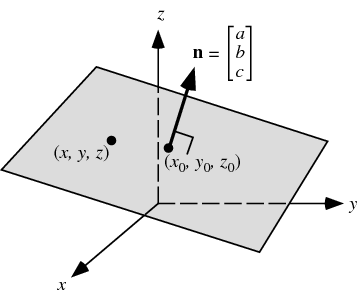
\includegraphics[width=.4\textwidth]{Figures/plane_n.png}
%        \end{figure}
%        \end{ex}
%        
%        Now, if we are given a surface (defined as a level surface or as the graph of a function), we can compute an approximation at a point called the \emph{tangent plane}.
%        
%        \begin{ex}{Tangent Plane to Paraboloid}
%        Consider the function 
%        \[
%        f(x,y)=-x^2-y^2.
%        \]
%        Then the graph of the function is given by plotting the points
%        \[
%        (x,y,f(x,y)).
%        \]
%        We compute the tangent plane by computing partial derivatives. We take
%        \begin{align*}
%        \frac{\partial f}{\partial x} &= -2x\\    
%        \frac{\partial f}{\partial y} &= -2y.
%        \end{align*}
%        Then the equation for a tangent plane at the point $(x_0,y_0,f(x_0,y_0))$ is given by
%        \[
%        z-f(x_0,y_0)=\partialx (x-x_0)+\partialy (y-y_0).
%        \]
%        So in our case, we have
%        \[
%        z-(-x_0^2-y_0^2)=-2x_0(x-x_0)-2y_0(y-y_0).
%        \]
%        Pictorially, it looks as follows (letting $p=(x_0,y_0,f(x_0,y_0))$):
%        \begin{figure}[H]
%            \centering
%            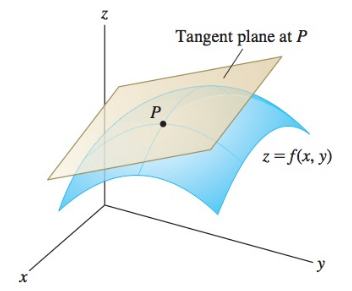
\includegraphics[width=.4\textwidth]{Figures/tangent-planes-1.png}
%        \end{figure}
%                
%        \end{ex}
%        
%        \begin{ex}{Tangent Vectors}{tangent_vectors}
%        Another way to understand this is to compute the \emph{tangent vectors} at a point. Take the same function $f(x,y)=-x^2-y^2$ and compute
%        \begin{align*}
%            \frac{\partial}{\partial x}\begin{bmatrix} x \\ y \\ f(x,y)\end{bmatrix} &= \begin{bmatrix} 1\\ 0 \\ -2x\end{bmatrix}\\
%            \frac{\partial}{\partial y}\begin{bmatrix} x \\ y \\ f(x,y)\end{bmatrix} &= \begin{bmatrix} 0\\ 1 \\ -2y\end{bmatrix}.
%        \end{align*}
%        Then take the cross product of these two vectors to get the normal vector to the tangent plane
%        \[
%        \begin{bmatrix} 1 \\ 0 \\-2x\end{bmatrix} \times \begin{bmatrix} 0 \\ 1 \\ -2y\end{bmatrix} = \begin{bmatrix} 2x \\ 2y \\ 1\end{bmatrix}.
%        \]
%        Pick a point $(x_0,y_0)$ and the normal to tangent plane is given by
%        \[
%        \mathbf{n}=\begin{bmatrix} 2x_0 \\ 2y_0 \\ 1 \end{bmatrix}.
%        \]
%        Which leads us to the following equation of a plane (but not exactly the tangent plane)
%        \[
%        2x_0 x + 2y_0y+z=0.
%        \]
%        This plane is parallel to the tangent plane and is often a nicer tool.
%        \end{ex}
%        
%        \begin{exercise}
%        Take the two equations for the planes above and simplify each to having a zero right hand side.  Then subtract each of these equations from each other and see what the difference is.
%        \end{exercise}
%        
%        
%%% START VEC FIELD
%        \section{The Jacobian of a Vector Field}
%        Recall we can define a three dimensional vector field $\mathbf{v}(x,y,z)$ by
%        \[
%        \mathbf{v}(x,y,z)=(v_1(x,y,z),v_2(x,y,z),v_3(x,y,z)) = \begin{bmatrix} v_1(x,y,z) \\ v_2(x,y,z) \\ v_3(x,y,z) \end{bmatrix}
%        \]
%        where we call each $v_1$, $v_2$, and $v_3$ the component functions.  Notice that each component function is a scalar function!
%        
%        Since each component function is a scalar function, we know how to compute the derivative of each by computing the gradient.  This gives us a way to then talk about the derivative of the vector field as a whole
%        
%        \begin{df}{Jacobian}{jacobian}
%        The \textbf{Jacobian} of a vector field $\mathbf{v}(x,y,z)$ is a matrix
%        \[
%        J(x,y,z)\coloneqq \begin{bmatrix} \nabla v_1^T \\ \nabla v_2^T \\ \nabla v_3^T \end{bmatrix},
%        \]
%        where the gradients are transposed (the superscript $T$) so they are are written as row vectors and placed in a matrix. More specifically, we can write this matrix as 
%        \[
%        J(x,y,z) = \begin{bmatrix} \frac{\partial v_1}{\partial x} & \frac{\partial v_1}{\partial y} & \frac{\partial v_1}{\partial z}\\ \frac{\partial v_2}{\partial x} & \frac{\partial v_2}{\partial y} & \frac{\partial v_2}{\partial z} \\ \frac{\partial v_3}{\partial x} & \frac{\partial v_3}{\partial y} & \frac{\partial v_3}{\partial z} \end{bmatrix}.
%        \]
%        \end{df}
%        
%        The Jacobian contains a lot of information. Intuitively, it tells us how each component of the vector field changes in each direction.  
%        
%        \begin{ex}{Computing the Jacobian, 1}{computing_jacobian}
%        Let us consider the vector field
%        \[
%        \mathbf{v}(x,y,z) = (x^2+y^2,z,x+y+z).
%        \]
%        Then we can write
%        \begin{align*}
%            v_1(x,y,z)&= x^2+y^2\\
%            v_2(x,y,z)&= z\\
%            v_3(x,y,z)&= x+y+z.
%        \end{align*}
%        So we compute the gradients of each
%        \begin{align*}
%            \nabla v_1 &= \begin{bmatrix} 2x \\ 2y \\ 0 \end{bmatrix}\\
%            \nabla v_2 &= \begin{bmatrix} 0 \\ 0 \\ 1 \end{bmatrix}\\
%            \nabla v_3 &= \begin{bmatrix} 1 \\ 1 \\ 1 \end{bmatrix}.
%        \end{align*}
%        So then the Jacobian is
%        \[as
%        J(x,y,z) = \begin{bmatrix} 2x & 2y & 0 \\ 0 & 0 & 1\\ 1 & 1 & 1 \end{bmatrix}.
%        \]
%        \end{ex}
%        
%        A related and important quantity comes in the form of the determinant of the Jacobian.  We've previously talked about the determinant of a matrix as telling us the (signed) scaling of volume of a linear transformation.  That is, for example, if we have
%        \[
%        A = \begin{bmatrix} 2 & 0 & 0\\ 0 & 2 & 0\\ 0 & 0 & 2 \end{bmatrix}
%        \]
%        then $\det(A)=8$ and we say that volumes of parallelopipeds are increased by a factor of $8$ in this case.  
%        
%        When you are given a vector field, you can think of different regions of space being stretched differently.  This is why we have that the Jacobian is a matrix that depends on the position $(x,y,z)$.  In this case, the volumes that are being stretched are very very tiny parallelopipeds.  You can think of cubes with side lengths $dx$, $dy$, and $dz$. 
%        
%        \begin{ex}{Computing the Jacobian, 2}
%        We found that given
%        \[
%        \mathbf{v}(x,y,z) = (x^2+y^2,z,x+y+z)
%        \]
%        that
%        \[
%        J(x,y,z) = \begin{bmatrix} 2x & 2y & 0 \\ 0 & 0 & 1 \\ 1 & 1 & 1 \end{bmatrix}
%        \]
%        As we can see, this matrix depends on position.  Let's compute the determinant
%        \[
%        |J(x,y,z)|=\det(J(x,y,z))=2(y-x). 
%        \]
%        Something weird seems to happen with $y=x$ as the determinant $|J(x,y,z)|$ will be zero in this case. Otherwise, things are fine.
%        \end{ex}
%        
%        \section{Divergence and Curl}
%        Often we do not need to use the whole Jacobian.  We will find it to be necessary for integration, however.  
%        
%        For analysis of vector fields, we often wish to break them into their smaller pieces.  Fundamentally, we can break vector fields into two parts:
%        \begin{itemize}
%            \item Sources and sinks,
%            \item Rotations.
%        \end{itemize}
%        
%        \subsubsection{Sources, Sinks, and Divergence Fields}
%        With some vector fields, we can make the analogy that some quantity (think air or water) is being added or removed from the system.  We call these \emph{sources} and \emph{sinks} respectively.  We want to quantify how much of some quantity is being added. This quantity is called the \emph{divergence}.
%        
%        Recall, we can write
%        \[
%        \nabla = \begin{bmatrix} \frac{\partial}{\partial x} \\ \frac{\partial}{\partial y} \\ \frac{\partial}{\partial z} \end{bmatrix}.
%        \]
%        If we are also given a vector field
%        \[
%        \mathbf{v}(x,y,z) = \begin{bmatrix} v_1(x,y,z) \\ v_2(x,y,z) \\ v_3(x,y,z) \end{bmatrix},
%        \]
%        we can compute the \textbf{divergence} of $\mathbf{v}$ by
%        \[
%        \nabla \cdot \mathbf{v}(x,y,z) = \frac{\partial v_1}{\partial x} + \frac{\partial v_2}{\partial y} + \frac{\partial v_3}{\partial z}.
%        \]
%        Notice that this quantity is a scalar!  This scalar value, the divergence, tells us how much the vector field is diverging at a point $(x,y,z)$. In other words, it tells us how much of a quanitity is being added or removed there.
%        
%        \begin{ex}{Source Field}{source_field}
%        Consider
%        \[
%        \mathbf{v}(x,y,z) = \begin{bmatrix} x \\ y \\ z \end{bmatrix}.
%        \]
%        Then the divergence is
%        \[
%        \nabla \cdot \mathbf{v}(x,y,z) = \frac{\partial v_1}{\partial x} + \frac{\partial v_2}{\partial y} + \frac{\partial v_3}{\partial z} = 1 + 1 + 1 = 3.
%        \]
%        We can think of a source of air being placed at each point that pumps in $3$ units of air per second, or specifically being pumped in at the origin. The vector field looks like:
%        \begin{figure}[H]
%            \centering
%            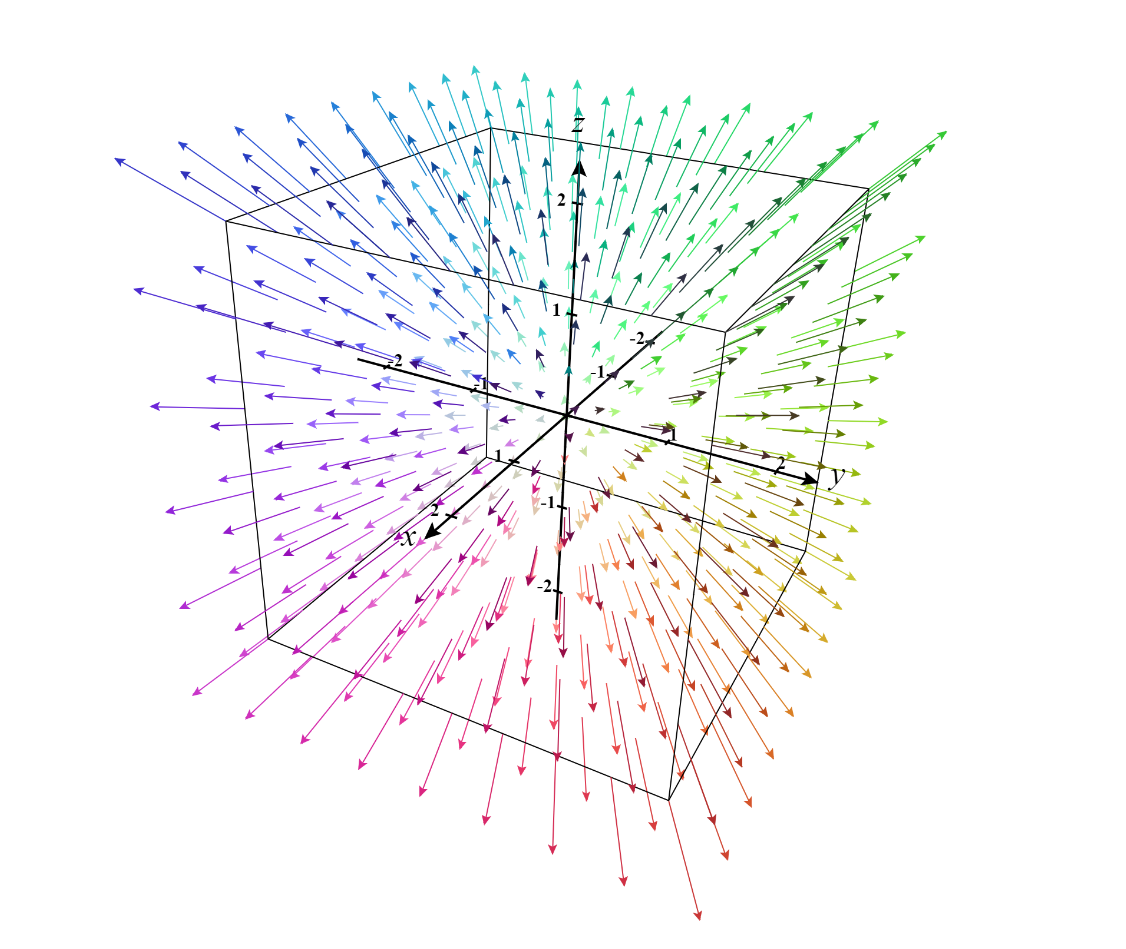
\includegraphics[width=.6\textwidth]{Figures/divergence_field.png}
%        \end{figure}
%        \end{ex}
%        
%        \subsubsection{Rotation Fields}
%        The divergence was the quantity that measured the outflow from a point for a vector field.  The other quantity we can measure is the rotation of a vector field at a point.
%        
%        We define the \textbf{curl} of a vector field $\mathbf{v}(x,y,z)$ to be
%        \[
%        \nabla \times \mathbf{v}(x,y,z) = \begin{bmatrix} \frac{\partial v_3}{\partial y} - \frac{\partial v_2}{\partial z} \\ \frac{\partial v_1}{\partial z} - \frac{\partial v_3}{\partial x} \\ \frac{\partial v_2}{\partial x} - \frac{\partial v_1}{\partial y} \end{bmatrix}.
%        \]
%        \emph{Note that the curl is a vector!} The curl is a vector that points orthogonally to the plane where rotation occurs and has magnitude relative to how quickly the field swirls.
%        
%        It's a bit involved to go through the work and see exactly why this is the correct quantity for seeing rotation of a vector field.  However, you can recall that the cross product was useful in describing rotational motion of rigid bodies (that is, it showed up in angular velocity/momentum).
%        
%        \begin{ex}{A Rotation Field}{rot_field}
%        Consider the vector field
%        \[
%        \mathbf{v}(x,y,z) = (-y,x,z)
%        \]
%        which looks like
%        \begin{figure}[H]
%            \centering
%            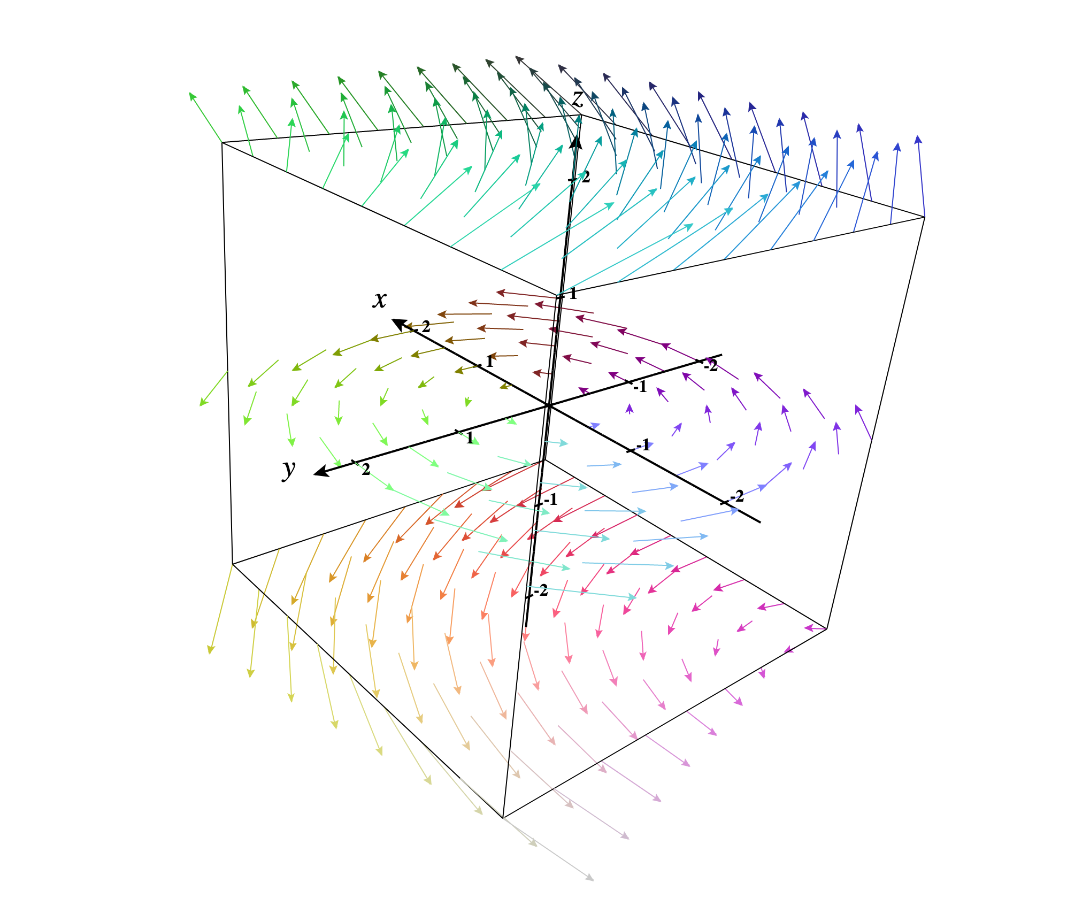
\includegraphics[width=.6\textwidth]{Figures/curl_field.png}
%        \end{figure}
%        We let
%        \begin{align*}
%            v_1(x,y,z) &= -y\\
%            v_2(x,y,z) &= x\\
%            v_3(x,y,z) &= z.
%        \end{align*}
%        If we look in this figure where $z=0$, we can clearly see that this field swirls around the origin.  If the curl is to measure rotation, we should see it nonzero here.
%        
%        Let us compute the curl of this field.  For this, we will all the other partial derivatives not contained in the divergence. That is, we need
%        \begin{align*}
%            \frac{\partial v_1}{\partial y} &= -1 & \frac{\partial v_1}{\partial z} &= 0\\
%            \frac{\partial v_2}{\partial x} &= 1& \frac{\partial v_2}{\partial z} &= 0\\
%            \frac{\partial v_3}{\partial x} &= 0 &  \frac{\partial v_3}{\partial y} &=0.
%        \end{align*}
%        Then we have
%        \[
%        \nabla \times \mathbf{v}(x,y,z) = \begin{bmatrix} 0-0\\ 0-0 \\ 1-(-1)\end{bmatrix} = \begin{bmatrix} 0\\ 0 \\ 2\end{bmatrix}.
%        \]
%        
%        We can decipher the meaning here by saying that the swirling occurs in planes parallel to the $xy$-plane since the direction of the curl is only in the $z$-direction.  That is, curl is pointing perpendicularly to the plane of rotation.  How quickly the field swirls is given by the magnitude of the curl which is $2$ in this case.  Using the right hand rule we discussed previously this tells us the direction of swirling as well.  We have swirling counter-clockwise in the planes parallel to the $xy$-plane, and so we expect the curl to point in the positive $z$-direction.
%        
%        Take a moment to analyze this using the figure provided or by plotting this yourself.
%        \end{ex}
%        
%        \begin{ex}{Divergence of the Rotation Field}
%        One may also consider the divergent nature of the field 
%        \[
%        \mathbf{v}(x,y,z) = (-y,x,z)
%        \]
%        from the previous example and find that 
%        \[
%        \nabla \cdot \mathbf{v}(x,y,z) = 1.
%        \]
%        So, there is in some way divergence as well.  This leads us to breaking the vector field into a part that swirls and a part that diverges as follows:
%        \begin{align*}
%            \mathbf{v}_\textrm{swirl}(x,y,z) &= (-y,x,0)\\
%            \mathbf{v}_\textrm{div}(x,y,z) &= (0,0,z).
%        \end{align*}
%        This type of analysis can be very helpful when considering real world problems.  It is especially important in electromagnetism.
%        \end{ex}
%        
%        \subsubsection{Constant Vector Fields}
%        Most of the understanding of vector fields was just covered by understanding the the part that diverges and the part that curls.  However, you can always add constants to these vector fields and these constants will not change the divergence or curl. Why? Take the following example.
%        
%        \begin{ex}{Constant Fields}{const_field}
%        Let 
%        \[
%        \mathbf{v}(x,y,z) = (c_1,c_2,c_3)
%        \]
%        where $c_1,c_2,$ and $c_3$ are constants.  Then we can compute the Jacobian of $\mathbf{v}$
%        \[
%        J(x,y,z) = \begin{bmatrix} 0 & 0 & 0 \\ 0 & 0 & 0\\ 0 & 0 &0 \end{bmatrix}.
%        \]
%        Since the Jacobian holds all the partial derivative information, we can know from this that 
%        \begin{align*}
%            \nabla \cdot \mathbf{v} &= 0\\
%            \nabla \times \mathbf{v} &= \mathbf{0}.
%        \end{align*}
%        \end{ex}
%        
%        \begin{exercise}
%        Specifically show that the divergence and curl of a constant vector field (as in the previous example) are zero.  
%        \end{exercise}
%        
%        All of this is to say that aside from the addition of a constant vector field, we understand the behavior by looking at divergence and curl.
%        
%        \section{The Laplacian of a Scalar Field}
%        In the study of partial differential equations (PDEs), we are often asked to find a function $u(x,y,z)$ that satisfies the following equation
%        \[
%        \nabla \cdot \nabla u(x,y,z) = f(x,y,z)
%        \]
%        for some given function $f(x,y,z)$.  We will revisit this Part III, but for now we should see exactly what we mean by
%        \[
%        \nabla \cdot \nabla u(x,y,z).
%        \]
%        
%        \begin{exercise}
%        Show that
%        \[
%        \nabla \cdot \nabla u(x,y,z) = \frac{\partial^2 u}{\partial x^2} + \frac{\partial^2 u}{\partial y^2} + \frac{\partial^2 u}{\partial z^2}.
%        \]
%        \end{exercise}
%        
%        \begin{df}{Laplacian}{laplacian}
%        We define the quantity
%        \[
%        \nabla \cdot \nabla u(x,y,z)
%        \]
%        to be the \textbf{Laplacian of $u(x,y,z)$} and we often write
%        \[
%        \Delta \coloneqq \nabla \cdot \nabla
%        \]
%        and call this the \textbf{Laplacian operator}.
%        \end{df}
%        
%        Intuitively, the Laplacian can be summed up in a few ways. 
%        \begin{itemize}
%            \item The Laplacian is the \emph{divergence} of the \emph{gradient} of a scalar function.
%            \item The Laplacian is the sum of ``curvatures" in each direction.
%        \end{itemize}
%        
%        \begin{ex}{Computing the Laplacian}{compute_laplacian}
%        Let us consider the functions
%        \[
%        f(x,y) = x^2+y^2
%        \]
%        and
%        \[
%        g(x,y) = x^2-y^2.
%        \]
%        Then we can compute the gradients of each function to get
%        \begin{align*}
%            \nabla f(x,y) &= \begin{bmatrix} 2x \\ 2y \end{bmatrix}\\
%            \nabla g(x,y) &= \begin{bmatrix} 2x \\ -2y \end{bmatrix}.
%        \end{align*}
%        We can then compute the divergence of each of these and find
%        \begin{align*}
%            \nabla \cdot \nabla f(x,y) &= 2+2 = 4\\
%            \nabla \cdot \nabla g(x,y) &= 2-2 =0.
%        \end{align*}
%        Let us see what these two functions look like to get a bit of an intuitive feel.
%        \begin{figure}[H]
%            \centering
%            \begin{subfigure}[h]{.45\textwidth}
%            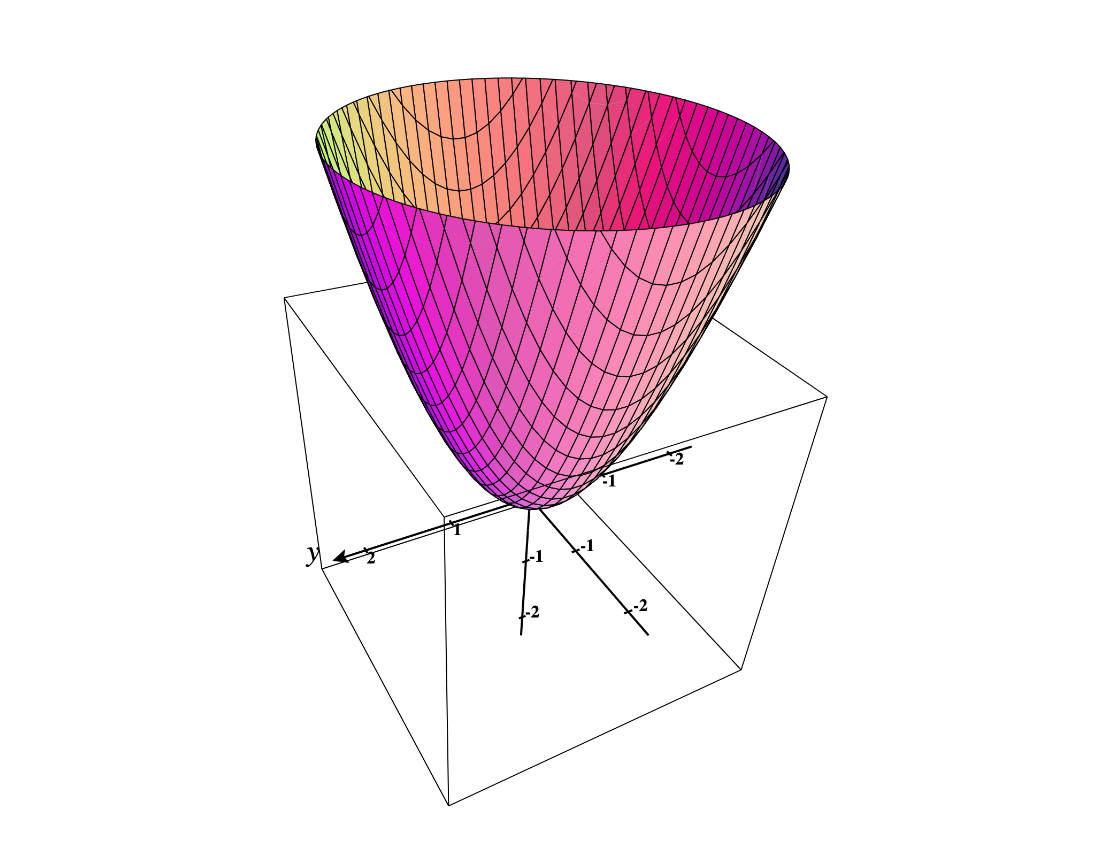
\includegraphics[width=\textwidth]{Figures/pos_laplace.png}
%            \caption{A plot of $f(x,y).$}
%            \end{subfigure}
%            ~
%            \begin{subfigure}[h]{.45\textwidth}
%            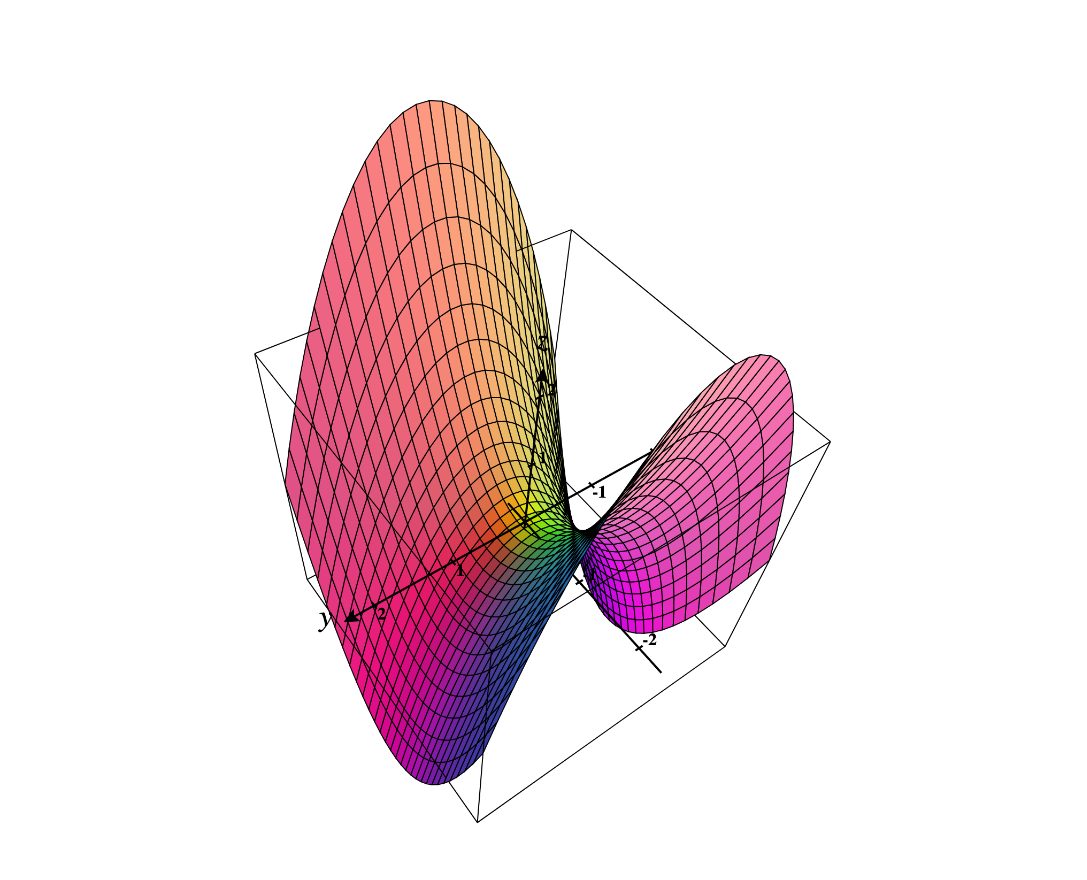
\includegraphics[width=\textwidth]{Figures/0_laplace.png}
%            \caption{A plot of $g(x,y).$}
%            \end{subfigure}
%        \end{figure}
%        Fundamentally we can see that these two functions are different.  It seems that for $f(x,y)$ we are curving upward in both the $x$ and $y$ direction which is what allows the Laplacian to be positive. However, for $g(x,y)$ one direction curves the opposite direction as the other which cancels out and gives us that the Laplacian is zero.  
%        
%        It turns out that the Laplacian describes many phenomenon. Two examples would be soap films and temperature flow.
%        \end{ex}
%
%        
%        We have covered all of the differential calculus of multivariate functions that we need.  That does not mean it won't show up again, but the material won't be new.  We now move onto integration in multiple dimensions.
%        
% %% MULTIVARIATE INTEGRATION       \chapter{Integration in Multiple Dimensions}
%        
%        \section{Integration of Scalar Fields}
%        
%        \subsubsection{One Dimensional Case}
%        In the case of one dimensional functions, we integrated to find the area under a curve.  That is, we were given a function $f(x)$ and asked to find
%        \[
%        \int_a^b f(x)dx
%        \]
%        which gave us the \emph{net} area under the curve.  Let's briefly review this with an example.
%        
%        \begin{ex}{One-Dimensional Integral}
%        Let $f(x) = x^2+2$, $a=1,$ and $b=2$. Then we want to find
%        \[
%        \int_a^b f(x)dx = \int_1^2 x^2+2dx.
%        \]
%        Then we use the \emph{Fundamental Theorem of Calculus}. So, we find the antiderivative of the integrand and evaluate at the endpoints as follows
%        \begin{align*}
%            \int_1^2 x^2+2dx &= \left[ \frac{x^3}{3}+2x\right]_1^2\\
%            &= \left(\frac{2^3}{3}+2(2)\right) - \left( \frac{1^3}{3}+2(1)\right)\\
%            &= \frac{13}{3}.
%        \end{align*}
%        \end{ex}
%        
%        \subsubsection{Two Dimensional Case}
%        
%        Say we are now given a function $f(x,y)$ and bounds on both the $x$ and $y$ by
%        $x_0 \leq x \leq x_1$ and $y_0 \leq y \leq y_1$.  We then wish to evaluate
%        \[
%        \int_{y_0}^{y_1} \int_{x_0}^{x_1} f(x,y)dxdy.
%        \]
%        You can think of this integral as being the \emph{net} volume under the surface given by $f(x,y)$.  
%        
%        How do we compute such an integral? The answer is iteratively.  Let's see how we do this with a concrete example.
%        
%        \begin{ex}{Two-Dimensional Integral}{2d_int}
%        Let $f(x,y)=xy$, $x_0=1$, $x_1=2$, $y_0=3$ and $y_1=4$.  So, we want to evaluate
%        \[
%        \int_{y_0}^{y_1}\int_{x_0}^{x_1} f(x,y)dxdy = \int_3^4 \int_1^2 xy dxdy.
%        \]
%        The way we do this is by first evaluating the integral with respect to $x$ (holding $y$ constant) and then integrate with respect to $y$ ($x$ will not appear here). So, we integrate from the inside out.  
%        
%        Let's start by integrating with respect to $x$. We take
%        \begin{align*}
%            \int_1^2 xy dx &= \left[ \frac{x^2y}{2}\right]_1^2\\
%            &= \left( y\frac{2^2}{2}\right) - \left(y\frac{1^2}{2}\right)\\
%            &=\frac{3}{2}y.
%        \end{align*}
%        Now we take this function of $y$, and we integrate this with the bounds we are given.  
%        \begin{align*}
%            \int_3^4 \frac{3}{2}y dy &= \left[ \frac{3y^2}{4} \right]_3^4\\
%            &= \frac{21}{4}.
%        \end{align*}
%        So we say that
%        \[
%        \int_3^4 \int_1^2 xy dxdy = \frac{21}{4}.
%        \]
%        
%        Let's walk through the steps again. We did
%        \begin{align*}
%            \int_{y_0}^{y_1} \int_{x_0}^{x_1} f(x,y)dxdy&= \int_3^4\int_1^2 xy dxdy\\
%            &= \int_3^4 \frac{3}{2}ydy \\
%            &= \frac{21}{4}.
%        \end{align*}
%        \end{ex}
%        
%        \subsubsection{Three Dimensional Case}
%        
%        Integration here is performed in the same way.  We are given a function $f(x,y,z)$ and bounds on $x$, $y$, and $z$ such as $x_0\leq x \leq x_1$, $y_0\leq y\leq y_1$, and $z_0\leq z \leq z_1$. Then we evaluate
%        \[
%        \int_{z_0}^{z_1}\int_{y_0}^{y_1}\int_{x_0}^{x_1} f(x,y,z)dxdydz.
%        \]
%        Let's work through an example.
%        
%        \begin{ex}{Three-Dimensional Integral}{3d_int}
%        Let
%        \[
%        f(x,y,z)=2x + 8xyz + 3,
%        \]
%        $x_0 = 0$, $x_1=1$, $y_0=2$, $y_1=3$, $z_0 =4$, $z_1=5$.  Then we want to find
%        \[
%        \int_{z_0}^{z_1}\int_{y_0}^{y_1}\int_{x_0}^{x_1} f(x,y,z)dxdydz = \int_4^5 \int_2^3 \int_0^1 2x+8xyz+3dxdydz.
%        \]
%        We do this iteratively.  So we first evaluate the $x$ integral holding the other variables constant for now.
%        \begin{align*}
%            \int_0^1 2x+8xyz+3 dx &= \left[ x^2 + 4x^2yz+3x\right]_0^1\\
%            &= \left( 1^2 + 4(1)^2yz+3(1)\right) - \left( 0^2+4(0)^2yz+3(0)\right)\\
%            &= 4yz+4.
%        \end{align*}
%        We then take this, and integrate with respect to $y$.
%        \begin{align*}
%            \int_2^3 4yz + 4 dy &= \left[ 2y^2z+4y\right]_2^3\\
%            &= (4(3)^2z+4(3))-(4(2)^2z+4(2))\\
%            &= 10z+4.
%        \end{align*}
%        Lastly, we integrate with respect to $z$
%        \begin{align*}
%            \int_4^5 10z+4 dz &= \left[ 5z^2+4z\right]_4^5\\
%            &= (5(5)^2+4(5))-(5(4)^2+4(4))\\
%            &=49.
%        \end{align*}
%        So we say that
%        \[
%        \int_4^5 \int_2^3 \int_0^1 2x+8xyz+3dxdydz = 49.
%        \]
%        Again, let's walk through the steps a bit
%        \begin{align*}
%            \int_{z_0}^{z_1}\int_{y_0}^{y_1}\int_{x_0}^{x_1} f(x,y,z)dxdydz &= \int_4^5 \int_2^3 \int_0^1 2x+8xyz+3dxdydz\\
%            &= \int_4^5 \int_3^4 4yz+4dydz\\
%            &= \int_4^5 10z+4dz\\
%            &= 49.
%        \end{align*}
%        \end{ex}
%        
%        \section{Antiderivatives}
%        In one variable calculus, we found that there is a relationship between the derivative and the indefinite integral.  In fact, this led us to call the indefinite integral the antiderivative.  This relationship was that
%        \[
%        \frac{d}{dx}\int f(x)dx = f(x)
%        \]
%        and
%        \[
%        \int \frac{df}{dx} = f(x) + C.
%        \]
%        From this, we realized that the indefinite integral is almost an inverse operation of the derivative.  It's just that in the case where we integrate a derivative, we only determine the function up to an additive constant. 
%        
%        \subsubsection{Potential Functions}
%        The higher dimensional analog happens to be a bit more nuanced but the idea remains the same. Let's say we are given a function $f(x,y,z)$ and we compute, for example,
%        \[
%        \partialx.
%        \]
%        The issue now becomes this.  Let's say that we let
%        \[
%        f(x,y,z) = x+yz.
%        \]
%        Then we have that
%        \[
%        \partialx = 1.
%        \]
%        The terms with just a $y,z$ dependence disappear.  So if we were to try to undo this with an integral, we find that 
%        \[
%        \int \partialx dx = \int 1 dx = x + g(y,z).
%        \]
%        That is to say, when we take an indefinite integral a multivariate function with respect to one variable, there could be a function of the residual variables that we cannot determine!
%        
%        \subsubsection{Integrating the Gradient}
%        
%        Let's say that we are given $\mathbf{v}(x,y,z)=\nabla f(x,y,z)$ and are asked to find the original function $f(x,y,z)$.  This problem is called finding the \textbf{potential function} for $\mathbf{v}$.  Remember that
%        \[
%        \nabla f(x,y,z) = \begin{bmatrix} \partialx \\ \partialy \\ \partialz \end{bmatrix}.
%        \]
%        What we do is the following.
%        \begin{enumerate}[1.]
%            \item We integrate $\partialx$ with respect to $x$ and determine $f(x,y,z)$ up to adding a function of only $y$ and $z$.  That is we are able to recover what is essentially a third of the potential function $f(x,y,z)$.
%            \item We integrate $\partialy$ with respect to $y$ and determine $f(x,y,z)$ up to adding a function of only $x$ and $z$.  
%            \item We integrate $\partialz$ with respect to $z$ and determine $f(x,y,z)$ up to adding a function of only $x$ and $z$.
%            \item Combine our knowledge from those three integrals we have determined $f(x,y,z)$ up to some additive constant!
%        \end{enumerate}
%        Let's work through an example.
%        
%        \begin{ex}{Finding a Potential Function}{find_potential}
%        Let's say that we are given the gradient of some function
%        \[
%        \nabla f(x,y,z) = \begin{bmatrix} y+z \\ x+z \\ x+y \end{bmatrix}.
%        \]
%        Then we follow the steps above
%        \begin{enumerate}[1.]
%            \item We integrate $\partialx$ with respect to $x$.  So we have
%            \begin{align*}
%                \int y+z dx &= xy+xz + g(y,z).
%            \end{align*}
%            Here, $g(y,z)$ is a function of just $y$ and $z$ that we cannot determine yet.
%            \item We integrate $\partialy$ with respect to $y$. So we have
%            \begin{align*}
%                \int x+z dy &= xy+yz + h(x,z).
%            \end{align*}
%            \item We integrate $\partialz$ with respect to $z$. So we have
%            \begin{align*}
%                \int x+y dz &= xz+yz + r(x,y).
%            \end{align*}
%            \item Now we know that all of these functions should be equal (up to a constant).  That is
%            \[
%            xy+xz+g(y,z)=xy+yz+h(x,z)=xz+yz+r(x,y).
%            \]
%            Here, we can see that $g(y,z)=yz$, $h(x,z)=xz$, and $r(x,y)=xy$.  So we have found that 
%            \[
%            f(x,y,z) = xy + xz + yz + C
%            \]
%            where the additive constant is there and is not something we can determine without a bit more information.
%        \end{enumerate}
%        \end{ex}
%        
%        \subsubsection{Requirements for Potentials}
%        
%        The main result here is the following.
%        
%        \begin{prop}{Curl of Gradient is Zero}{curl_of_gradient}
%        We have that
%        \[
%        \nabla \times \nabla f(x,y,z) = \mathbf{0}
%        \]
%        for all $f(x,y,z)$.
%        \end{prop}
%        
%        Then with a bit more work, one can show this follows.
%        
%        \begin{thm}{Potential $\iff$ Curl Free}{potential_curl_free}
%        Let $\mathbf{v}(x,y,z)$ be a vector field.  Then if 
%        \[
%        \nabla \times \mathbf{v} = \mathbf{0},
%        \]
%        then $\mathbf{v}(x,y,z) = \nabla f(x,y,z)$.  That is, a curl-free vector field $\mathbf{v}$ is really the gradient of some scalar function $f(x,y,z)$.  We call this scalar function $f$ the \textbf{potential} for $\mathbf{v}$.
%        \end{thm}
%        
%        This is what allows one to define the \emph{voltage} in electrostatics.  When charges are not moving, we have that the electric field $\mathbf{E}$ satisfies
%        \[
%        \nabla \times \mathbf{E} = \mathbf{0}
%        \]
%        and so it follows that
%        \[
%        \nabla V(x,y,z) = \mathbf{E}
%        \]
%        where $V$ is the potential.  We often call this electrostatic potential the voltage.



%\chapter{Differential Operators}

%\chapter{Integration}

%\part{Partial Differential Equations}





%\chapter{Remarks for Math 271}
%So far, we have covered a broad spectrum of topics. Many of these topics are not typical for a calculus II student, while some were.  Instead of taking the typical path through calculus II, then calculus III, we are venturing in a way that allows us to tell a story and build a firm foundation in mathematics specifically used throughout chemistry (and especially physical chemistry).  Typically, students in the calculus sequence learn differentiation and integration in a first course.  In a second course, students learn about sequences, series, power series, and Taylor series.  The third course entails learning calculus in higher dimensions. Specifically, one concentrates on calculus in 3-dimensional space since this is (arguably) the most physically meaningful to us.  Following the calculus sequence comes a course in differential equations where students are granted a handbook of techniques for solving different types of equations.

We approached this in a completely different way.  We began by studying complex numbers as this field of numbers allows us to factor polynomials.  The complex numbers also formed a vector space, and we briefly investigated this structure.  However, the main goal was to use these complex numbers in order to be able to solve many different first and second order differential equations.  These differential equations arose by studying systems that change over time. For example, we saw the harmonic oscillator equation arise from a spring/mass system. We also saw that chemical reactions were nicely described by differential equations. Those equations were describing systems that evolved over time and were given with initial function values at time zero. Another way differential equations arose was via boundary value problems. In particular, we studied the free particle in a one-dimensional box and came across many new concepts that resurface later.

Quickly, one sees that the techniques we used to solve differential equations were not all powerful. Thus, we sought out a new technique to solve more equations.  Eventually, we arrived at power series which provided us with newfound abilities to compute.  For example, one needs a tool such as a power series to compute values to the function $\sin(x)$!  Power series then proved as indispensable tools for solving more differential equations than we were previously able to work with.  When we still had trouble with a specific equation, we could then use a Taylor series to find polynomial approximations of terms in a differential equation and from there we could solve this equation using power series.  This part of the class was closer to a typical calculus II course but came with the added bonus of solving differential equations as well.  Even in a first course on ordinary differential equations, one may not solve equations using a power series! 

Finally, the last portion of this class came as a preparation to deal with higher dimensional spaces.  Understanding vector spaces and how they transform is a necessary building block to studying calculus in higher dimensions.  However, linear algebra can be done in more generality than we have covered here.  In this generality, we can see how topics we have previously worked with fit in as well.  For example, we spoke of linear differential equations and one can show that the set of solutions to a linear differential equation forms a vector space! Either way, the lessons that linear algebra teaches us about geometry and using geometrical tools to solve problems is highly important.  This can lead one to considering abstracting algebra further and seeing if that can help solve problems as well.  

Next, we move onto the sequel of Math 271 which is Math 272 where we will spend time learning calculus in higher dimensions.  In order to model the physical world, this is completely necessary.   The topics covered in 271 will lead straight into the new mathematics awaiting us in 272.  Keep these previous chapters as a reference as they are now prerequisite material!


 
\newenvironment{changemargin}[1]{%
\begin{list}{}{%
\setlength{\topsep}{#1}
\setlength{\listparindent}{\parindent}%
\setlength{\itemindent}{\parindent}%
\setlength{\parsep}{\parskip}%
}%
\item[]}{\end{list}}

\begin{changemargin}{0cm}
\printindex 
\end{changemargin}

 
\end{document}